\documentclass[hide notes,intlimits]{beamer}


\mode<presentation>
{
  \usetheme{UAFshade}
  \setbeamercovered{transparent}
}

% load packages
\usepackage{multimedia}
\usepackage{animate}
\usepackage[english]{babel}
\usepackage[latin1]{inputenc}
\usepackage[T1]{fontenc}
\usepackage{lmodern}
\usepackage[multidot]{grffile}
\usepackage[amssymb]{SIunits}

\usepackage{tikz}
\usetikzlibrary{shapes,arrows,shadows, calc}

\usepackage{pgfpages}
\setbeamertemplate{note page}[plain]
\setbeameroption{show notes on second screen=right}


\definecolor{dark red}{HTML}{E41A1C}
\definecolor{dark green}{HTML}{4DAF4A}
\definecolor{dark violet}{HTML}{984EA3}
\definecolor{dark blue}{HTML}{084594}
\definecolor{dark orange}{HTML}{FF7F00}
\definecolor{white}{HTML}{FFFFFF}
\definecolor{light blue}{HTML}{377EB8}
\definecolor{light red}{HTML}{FB9A99}
\definecolor{light violet}{HTML}{CAB2D6}

\definecolor{uaf red}{HTML}{E41A1C}
\definecolor{uaf blue}{HTML}{377EB8}
\definecolor{uaf green}{HTML}{4DAF4A}
\definecolor{uaf violet}{HTML}{984EA3}
\definecolor{uaf orange}{HTML}{FF7F00}
\setbeamercolor{boxed}{fg=black,bg=uaf yellow}


% Define block styles
\tikzstyle{initialization} = [ellipse, draw, 
    text badly centered, draw=dark violet,
        % The filling: 
        top color=white, 
        bottom color=dark violet]
\tikzstyle{initialization faded} = [ellipse, draw, 
    text badly centered, draw=dark violet!50,
        % The filling: 
        top color=white, 
        bottom color=dark violet!25]
\tikzstyle{hindcast} = [ellipse, draw,
    text badly centered, rounded corners,draw=dark orange,
        % The filling: 
        top color=white, 
        bottom color=dark orange]
\tikzstyle{hindcast faded} = [ellipse, draw,
    text badly centered, rounded corners,draw=dark orange!50,
        % The filling: 
        top color=white, 
        bottom color=dark orange!25]
\tikzstyle{forecast} = [ellipse, draw,
    text badly centered, rounded corners,draw=dark blue,
        % The filling: 
        top color=white, 
        bottom color=dark blue]
\tikzstyle{forecast faded} = [ellipse, draw,
    text badly centered, rounded corners,draw=dark blue!50,
        % The filling: 
        top color=white, 
        bottom color=dark blue!50]
\tikzstyle{arrow line} = [draw, -latex']
\tikzstyle{line} = [draw]



\graphicspath{{figures/}}

\setbeamerfont{caption}{size=\scriptsize}

% code adapted from http://tex.stackexchange.com/a/11483/3954

% some parameters for customization
\def\shadowshift{3pt,-3pt}
\def\shadowradius{6pt}

\colorlet{innercolor}{black!60}
\colorlet{outercolor}{gray!05}

% this draws a shadow under a rectangle node
\newcommand\drawshadow[1]{
    \begin{pgfonlayer}{shadow}
        \shade[outercolor,inner color=innercolor,outer color=outercolor] ($(#1.south west)+(\shadowshift)+(\shadowradius/2,\shadowradius/2)$) circle (\shadowradius);
        \shade[outercolor,inner color=innercolor,outer color=outercolor] ($(#1.north west)+(\shadowshift)+(\shadowradius/2,-\shadowradius/2)$) circle (\shadowradius);
        \shade[outercolor,inner color=innercolor,outer color=outercolor] ($(#1.south east)+(\shadowshift)+(-\shadowradius/2,\shadowradius/2)$) circle (\shadowradius);
        \shade[outercolor,inner color=innercolor,outer color=outercolor] ($(#1.north east)+(\shadowshift)+(-\shadowradius/2,-\shadowradius/2)$) circle (\shadowradius);
        \shade[top color=innercolor,bottom color=outercolor] ($(#1.south west)+(\shadowshift)+(\shadowradius/2,-\shadowradius/2)$) rectangle ($(#1.south east)+(\shadowshift)+(-\shadowradius/2,\shadowradius/2)$);
        \shade[left color=innercolor,right color=outercolor] ($(#1.south east)+(\shadowshift)+(-\shadowradius/2,\shadowradius/2)$) rectangle ($(#1.north east)+(\shadowshift)+(\shadowradius/2,-\shadowradius/2)$);
        \shade[bottom color=innercolor,top color=outercolor] ($(#1.north west)+(\shadowshift)+(\shadowradius/2,-\shadowradius/2)$) rectangle ($(#1.north east)+(\shadowshift)+(-\shadowradius/2,\shadowradius/2)$);
        \shade[outercolor,right color=innercolor,left color=outercolor] ($(#1.south west)+(\shadowshift)+(-\shadowradius/2,\shadowradius/2)$) rectangle ($(#1.north west)+(\shadowshift)+(\shadowradius/2,-\shadowradius/2)$);
        \filldraw ($(#1.south west)+(\shadowshift)+(\shadowradius/2,\shadowradius/2)$) rectangle ($(#1.north east)+(\shadowshift)-(\shadowradius/2,\shadowradius/2)$);
    \end{pgfonlayer}
}

% create a shadow layer, so that we don't need to worry about overdrawing other things
\pgfdeclarelayer{shadow} 
\pgfsetlayers{shadow,main}

\newsavebox\mybox
\newlength\mylen

\newcommand\shadowimage[2][]{%
\setbox0=\hbox{\includegraphics[#1]{#2}}
\setlength\mylen{\wd0}
\ifnum\mylen<\ht0
\setlength\mylen{\ht0}
\fi
\divide \mylen by 120
\def\shadowshift{\mylen,-\mylen}
\def\shadowradius{\the\dimexpr\mylen+\mylen+\mylen\relax}
\begin{tikzpicture}
\node[anchor=south west,inner sep=0] (image) at (0,0) {\includegraphics[#1]{#2}};
\drawshadow{image}
\end{tikzpicture}}

\newcommand\shadowimagec[3][]{%
\setbox0=\hbox{\includegraphics<#1>[#2]{#3}}
\setlength\mylen{\wd0}
\ifnum\mylen<\ht0
\setlength\mylen{\ht0}
\fi
\divide \mylen by 120
\def\shadowshift{\mylen,-\mylen}
\def\shadowradius{\the\dimexpr\mylen+\mylen+\mylen\relax}
\begin{tikzpicture}
\node[anchor=south west,inner sep=0] (image) at (0,0) {\includegraphics<#1>[#2]{#3}};
\drawshadow{image}
\end{tikzpicture}}


\newenvironment{transbox}[1][]{%
\begin{tikzpicture}
\node[drop shadow,rounded corners,text width=\textwidth,fill=white, fill opacity=#1,text opacity=1] \bgroup
}{
\egroup;\end{tikzpicture}} 

\newenvironment{transbox-tight}{%
\begin{tikzpicture}
\node[drop shadow,rounded corners,fill=uaf yellow, fill opacity=0.75,text opacity=1] \bgroup
}{
\egroup;\end{tikzpicture}} 


% title page
\title[] % (optional, use only with long paper titles)
{Glaciers: The Biggest Losers}



\author[Aschwanden] % (optional, use only with lots of authors)
{Andy Aschwanden}
% - Give the names in the same order as the appear in the paper.
% - Use the \inst{?} command only if the authors have different
%   affiliation.

\institute[Geophysical Institute] % (optional, but mostly needed)
{Geophysical Institute}
% - Use the \inst command only if there are several affiliations.
% - Keep it simple, no one is interested in your street address.


\date{}

\begin{document}

% define what is shown at the beginning of each section
\AtBeginSection[]
{
  \begin{frame}<handout:0>
    \frametitle{Outline}
   \tableofcontents[currentsection,subsectionstyle=hide/hide/hide]
  \end{frame}
}

% define what is shown at the beginning of each subsection
\AtBeginSubsection[]
{
 \begin{frame}<beamer>
  \frametitle{Outline}
   \tableofcontents[currentsection,currentsubsection]
 \end{frame}
}


\setbeamertemplate{background canvas}
  {
     \tikz{\node[inner sep=0pt,opacity=1.] {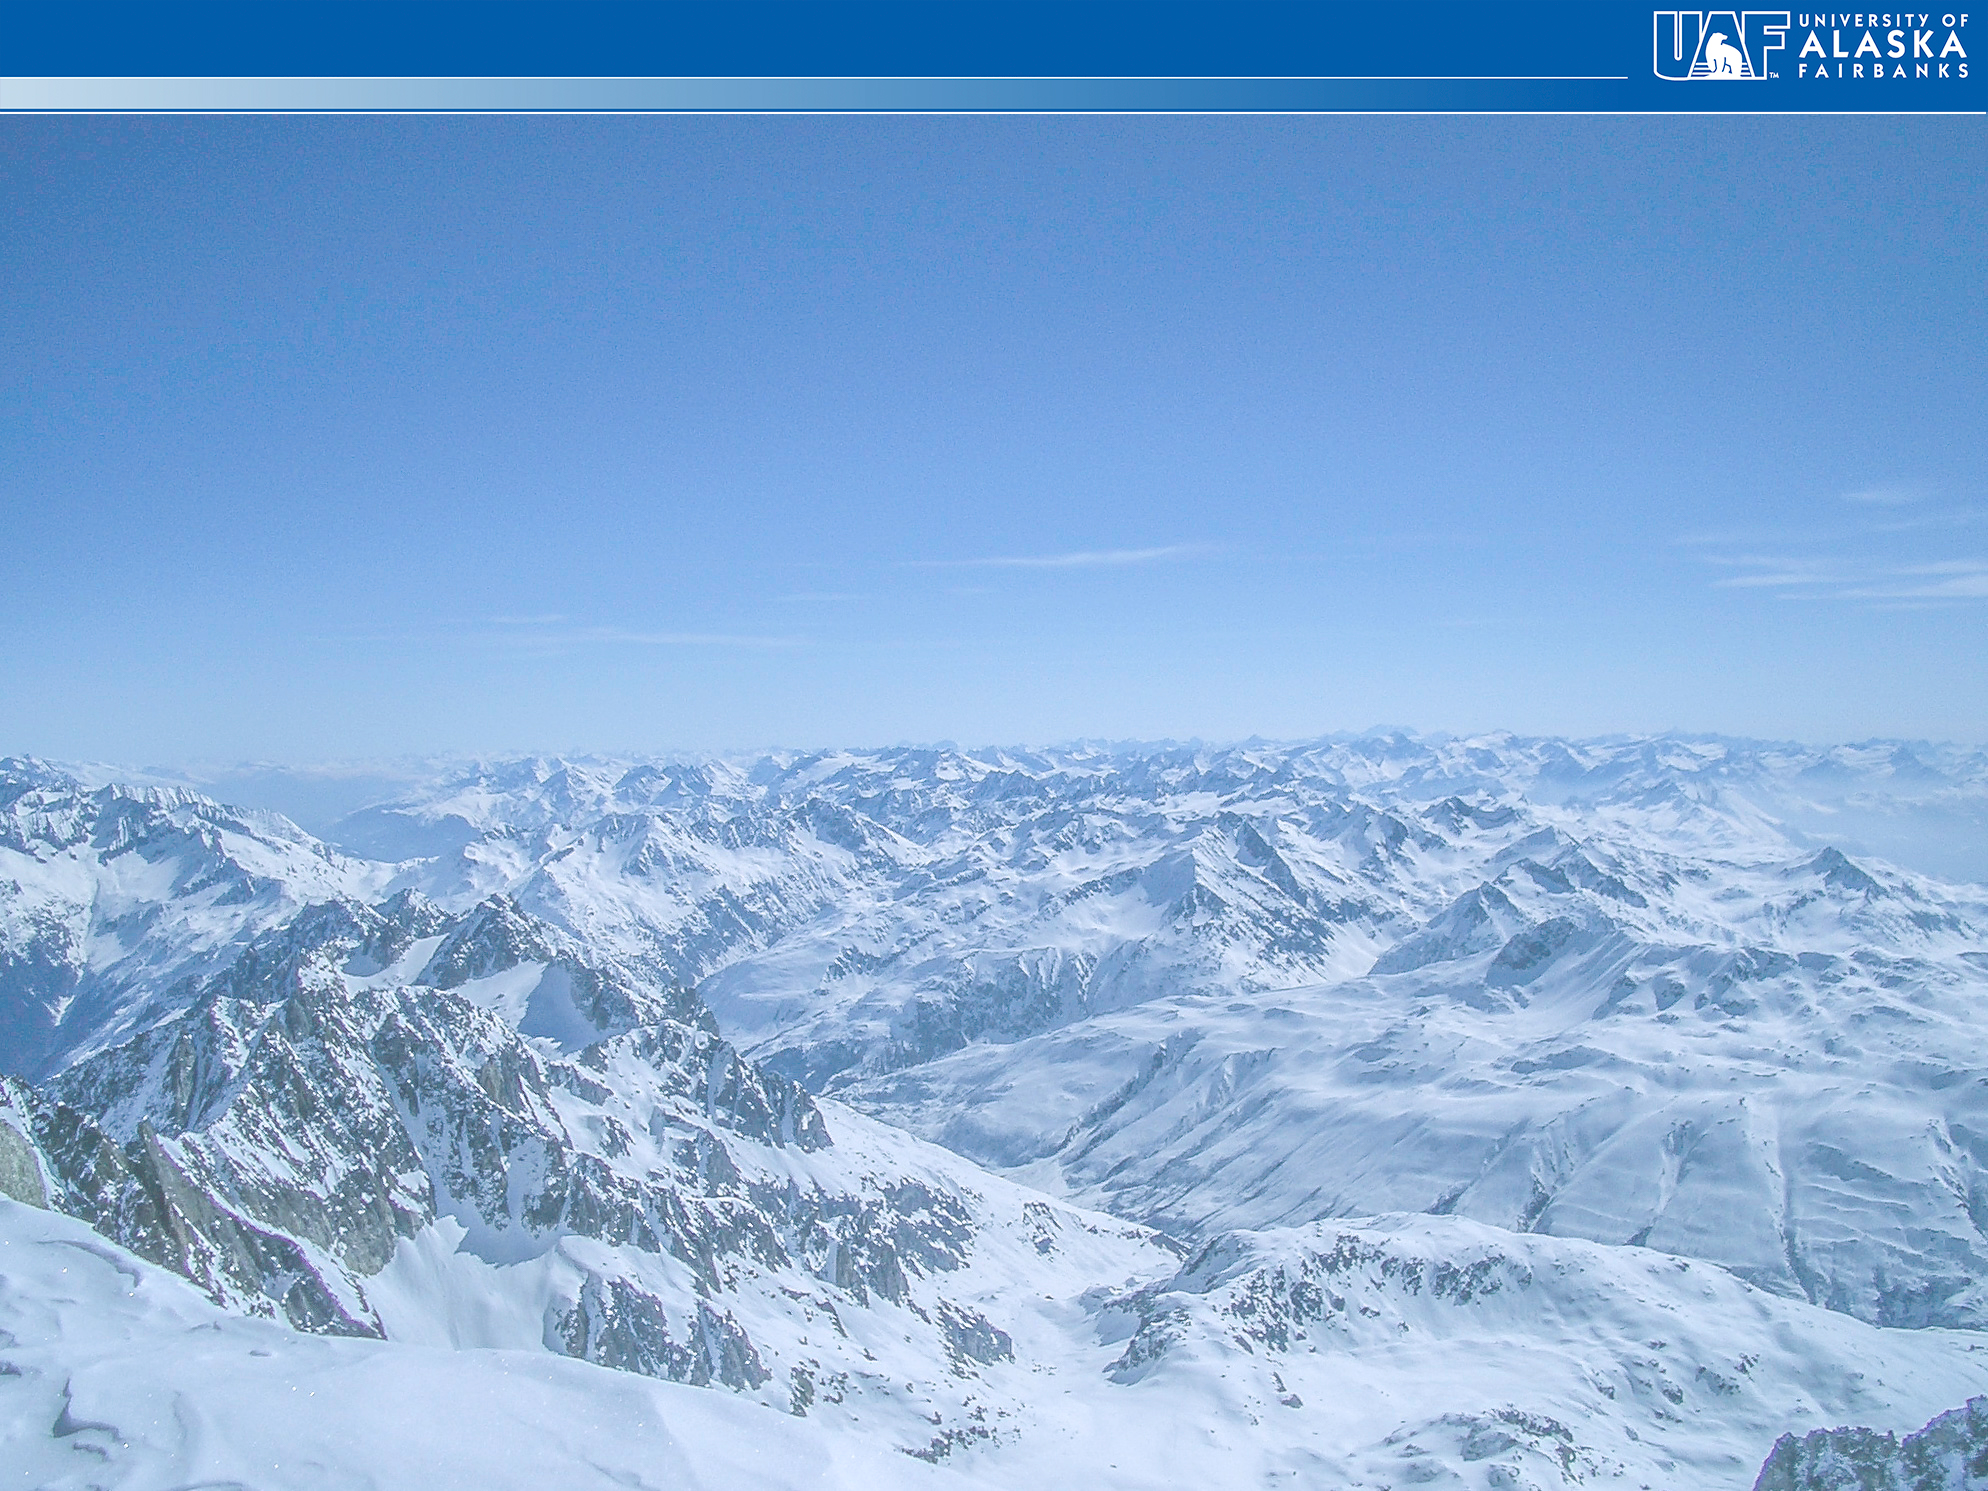
\includegraphics[width=\paperwidth]{galenstock_bg}};}
}


% insert titlepage
\begin{frame}
  \titlepage
  \note[item]{Who has ever seen a glacier?}
  \note[item]{Who has ever set foot on a glacier?}
  \note[item]{The picture here shows the view from on of my favorite places}
\end{frame}

\setbeamertemplate{background canvas}
  {
} 


\setbeamertemplate{background canvas}
  {
     \tikz{\node[inner sep=0pt,opacity=1.] {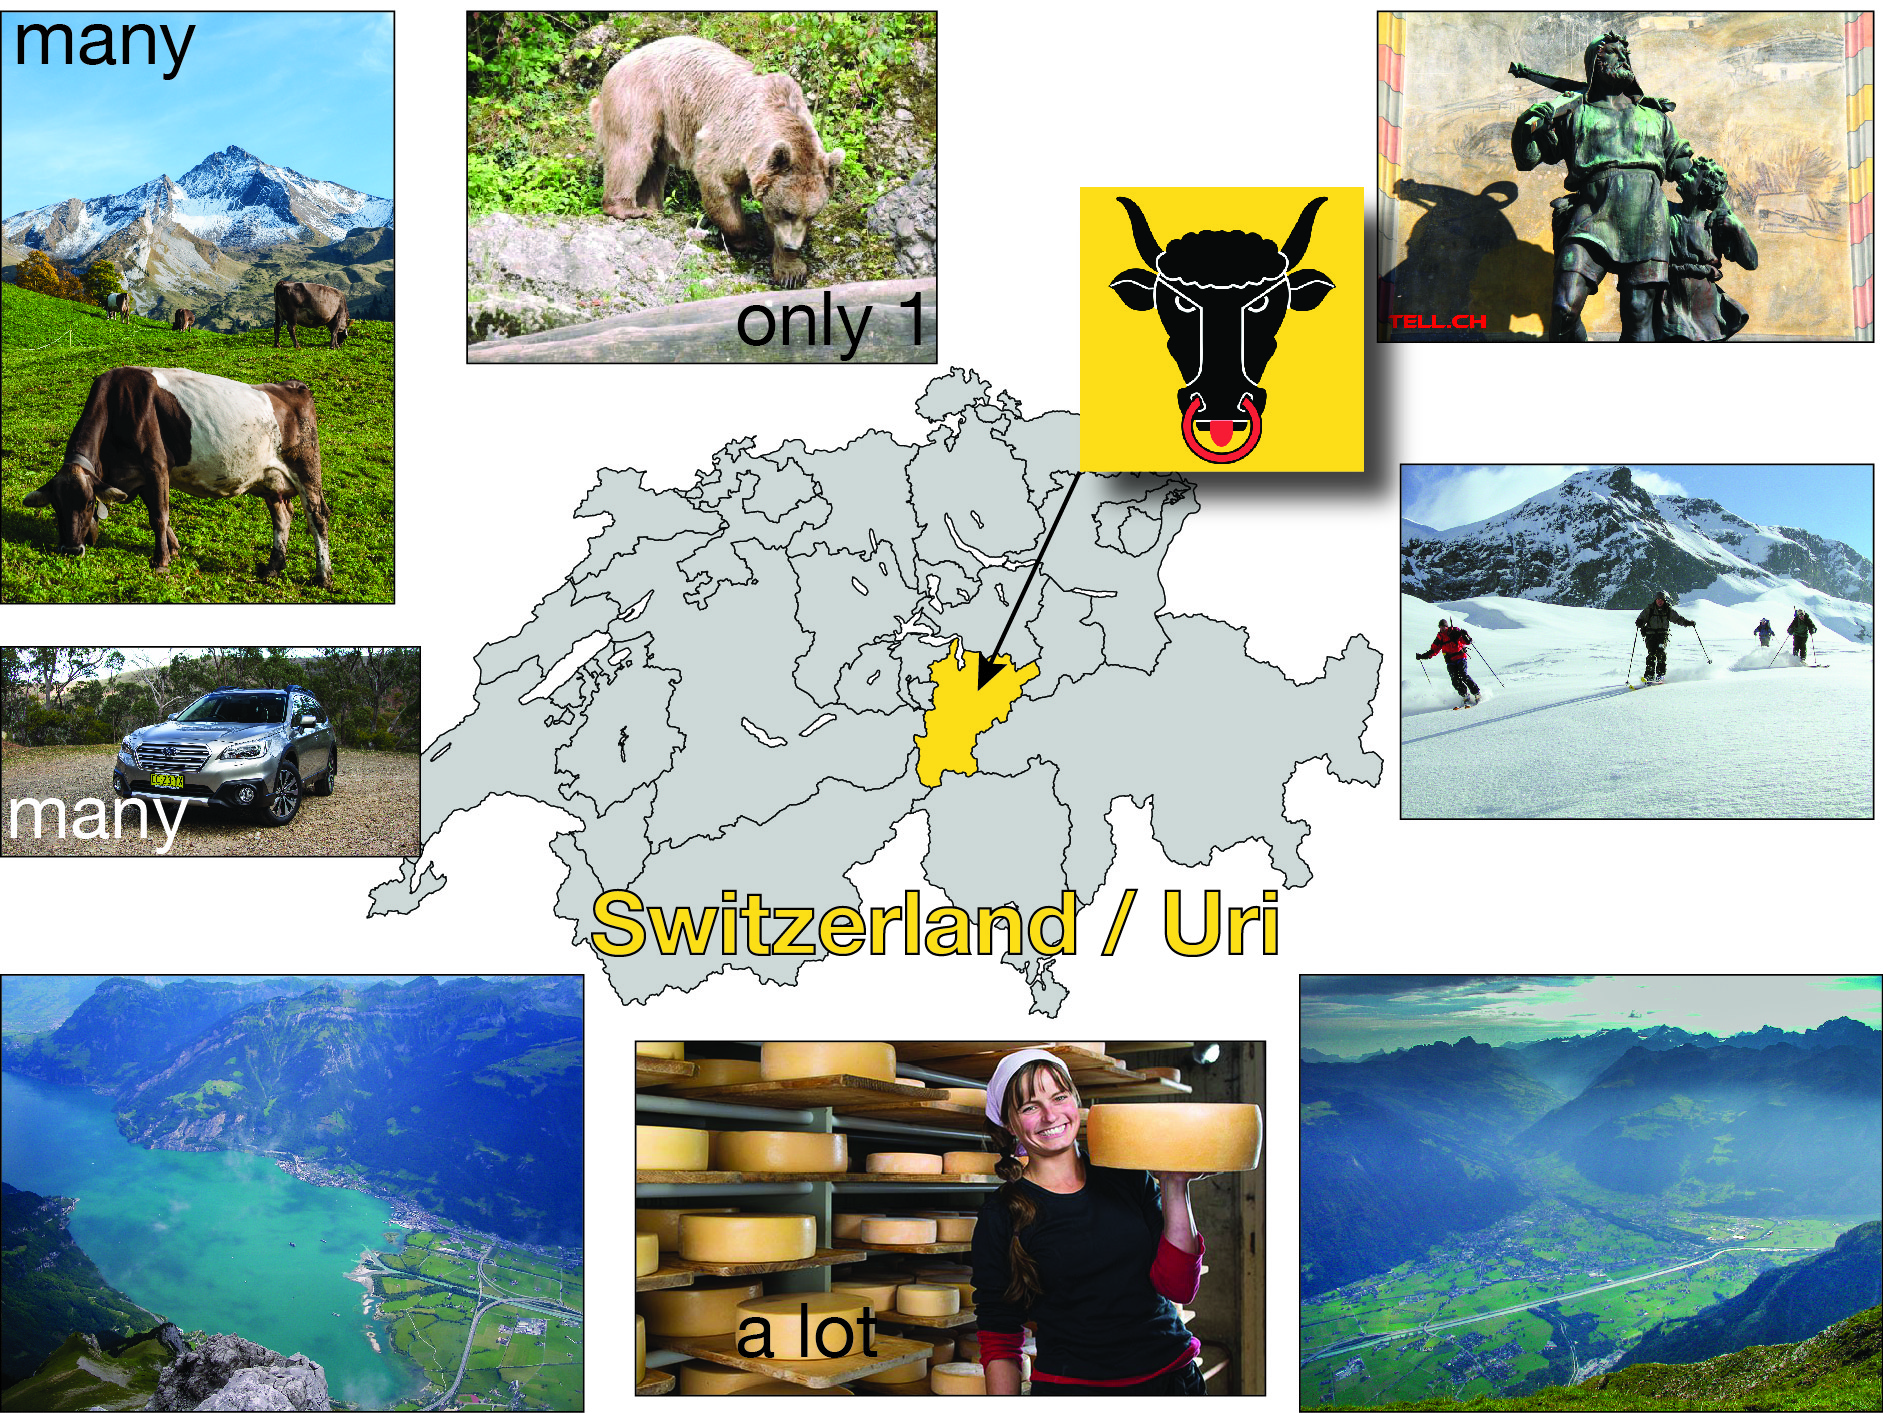
\includegraphics[width=\paperwidth]{uri-collage}};}
}

\begin{frame}[plain]
  \note[item]{I grew up in Switzerland, in the Kanton Uri---a Kanton is the equivalent to a State}
  \note[item]{True to the stereotype, we have many cows in Uri and produce a lot of good cheese}
  \note[item]{Last year we had on bear roaming through Uri, which gave it some Alaska-feel}
  \note[item]{According to legend, William Tell was born in Uri, who freed us from the Austrian oppression in 1291}
  \note[item]{We also have a lot of mountains to climb and to ski}
\end{frame}

\setbeamertemplate{background canvas}
{
  \tikz{\node[inner sep=0pt,opacity=1.] {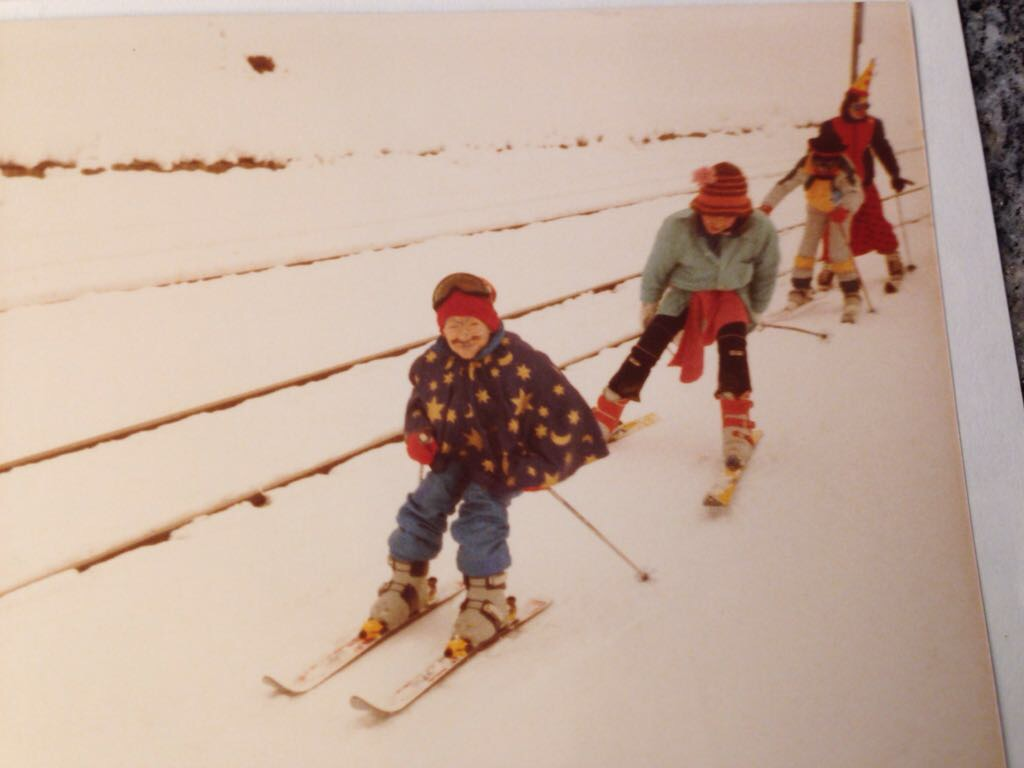
\includegraphics[width=\paperwidth]{andy-ski}};}
}

\begin{frame}[plain]
  \note[item]{So no surprise}
  \note[item]{I grew up on skis, I learned to downhill ski right after learning to walk}
  \note[item]{In Switzerland ``skiing'' always means downhill skiing, unlike here in Fairbanks where skiing usually means XC skiing}
\end{frame}



\setbeamertemplate{background canvas}
{
  \tikz{\node[inner sep=0pt,opacity=1.] {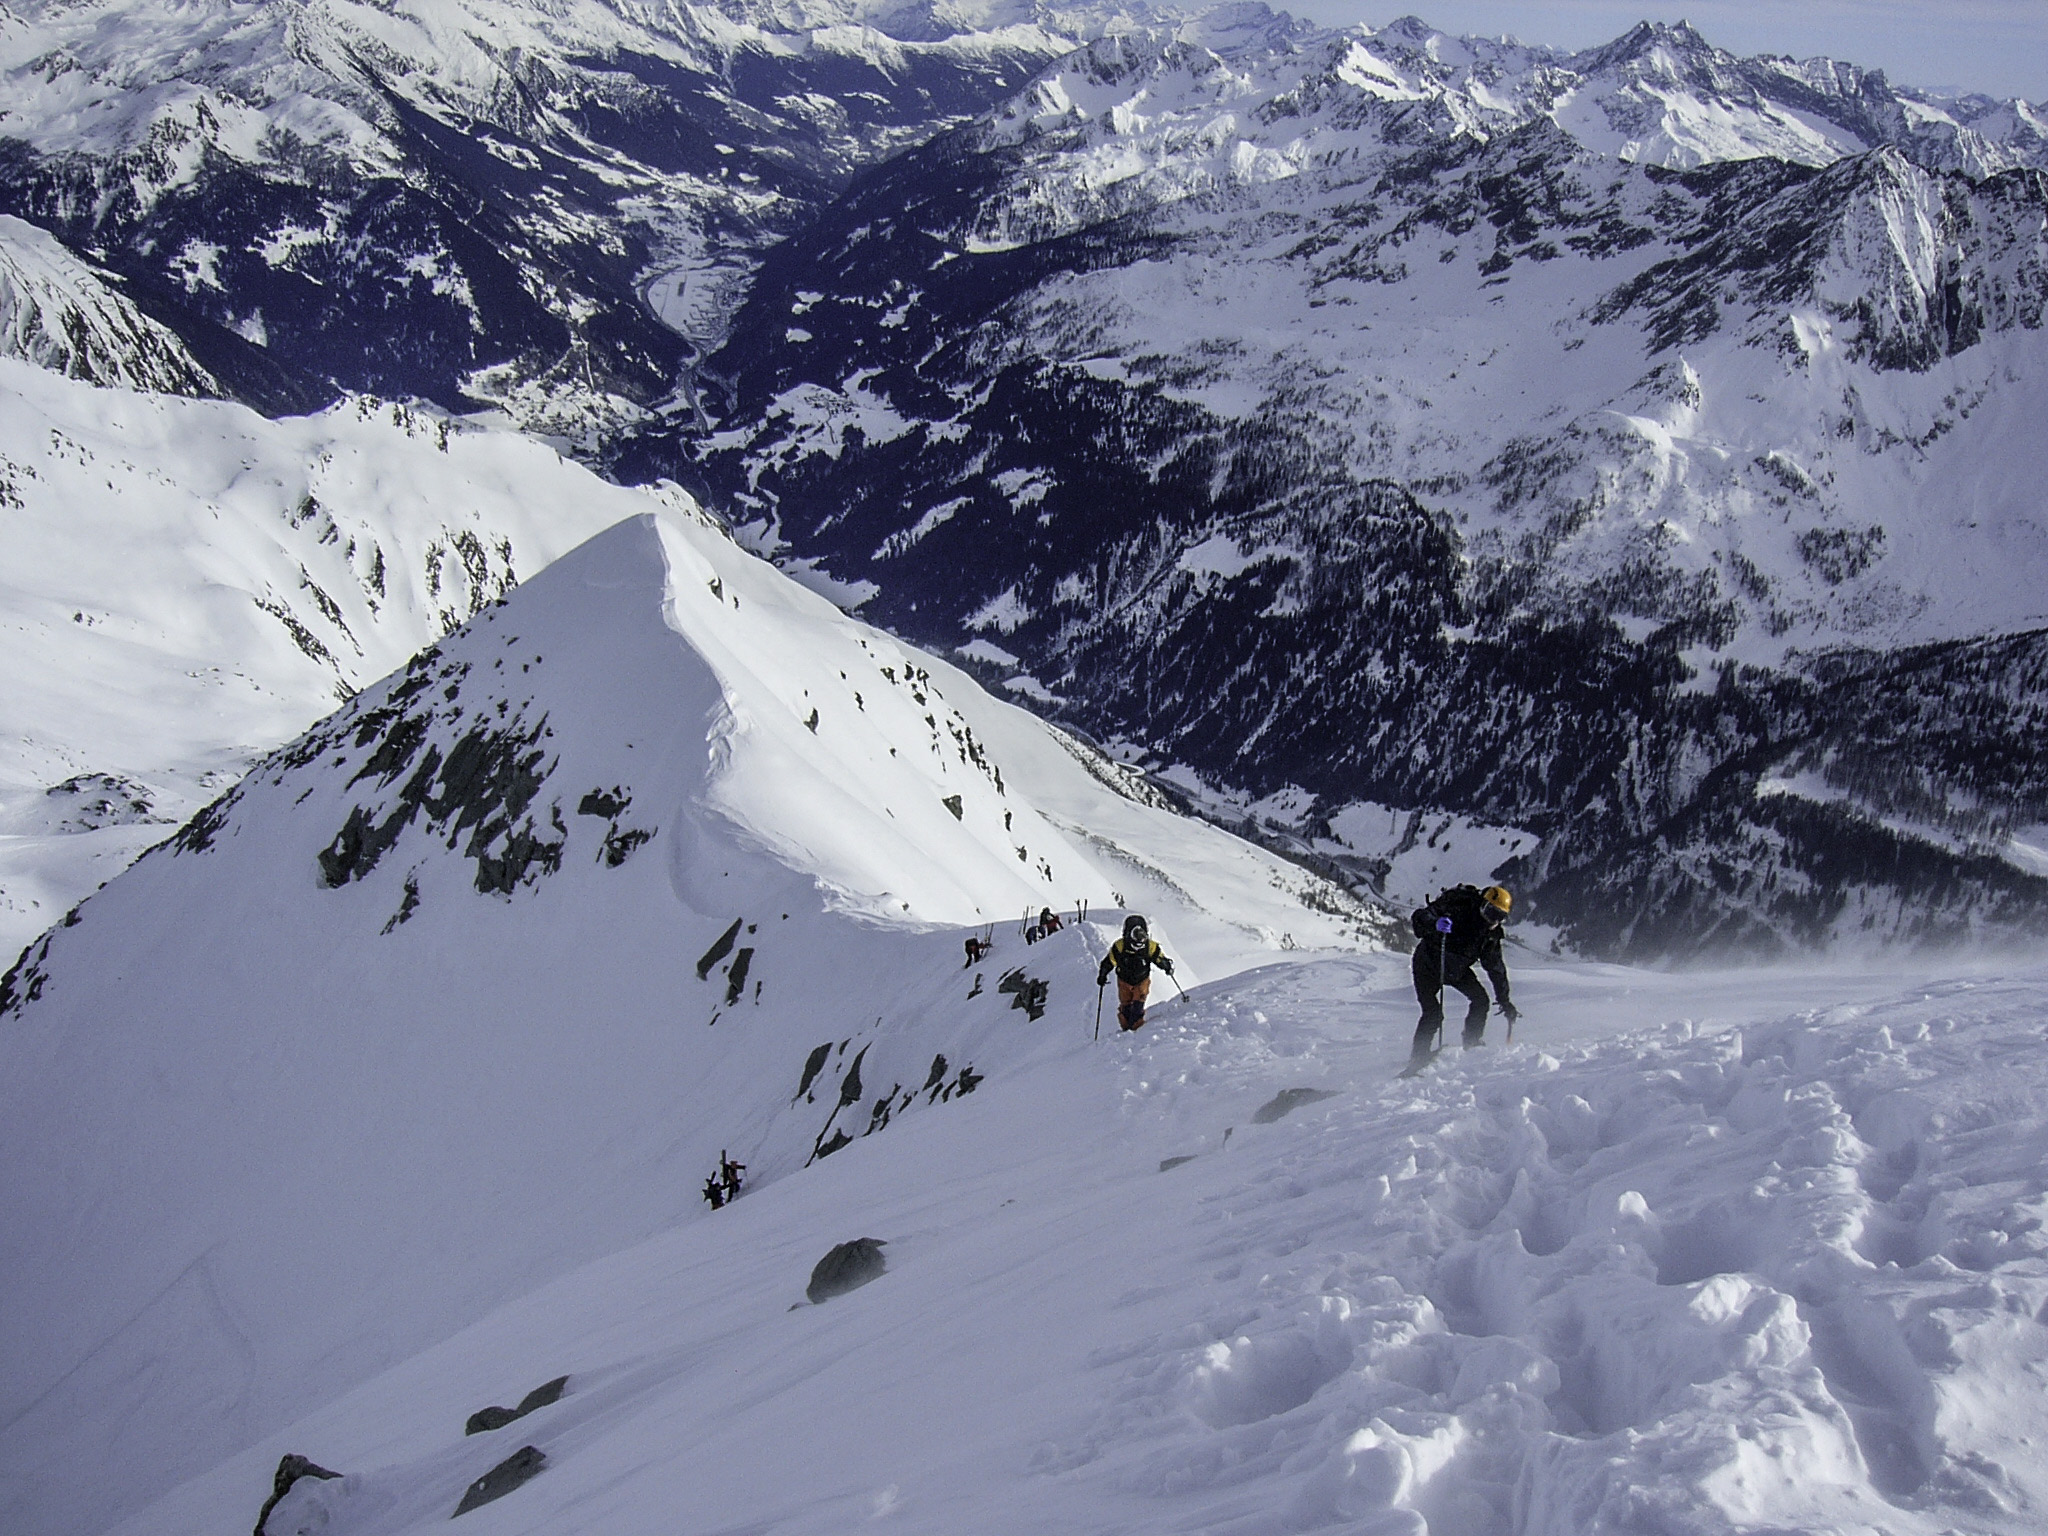
\includegraphics[width=\paperwidth]{ski-climb}};}
}

\begin{frame}[plain]
  \note[item]{When I was a bit older, I became tired of waiting for the next gondola}
  \note[item]{so started with ski mountaineering}
  \note[item]{and while spending my weekends in the mountains, I started to notice change}
\end{frame}

\setbeamertemplate{background canvas}
{
  \tikz{\node[inner sep=0pt,opacity=1.] {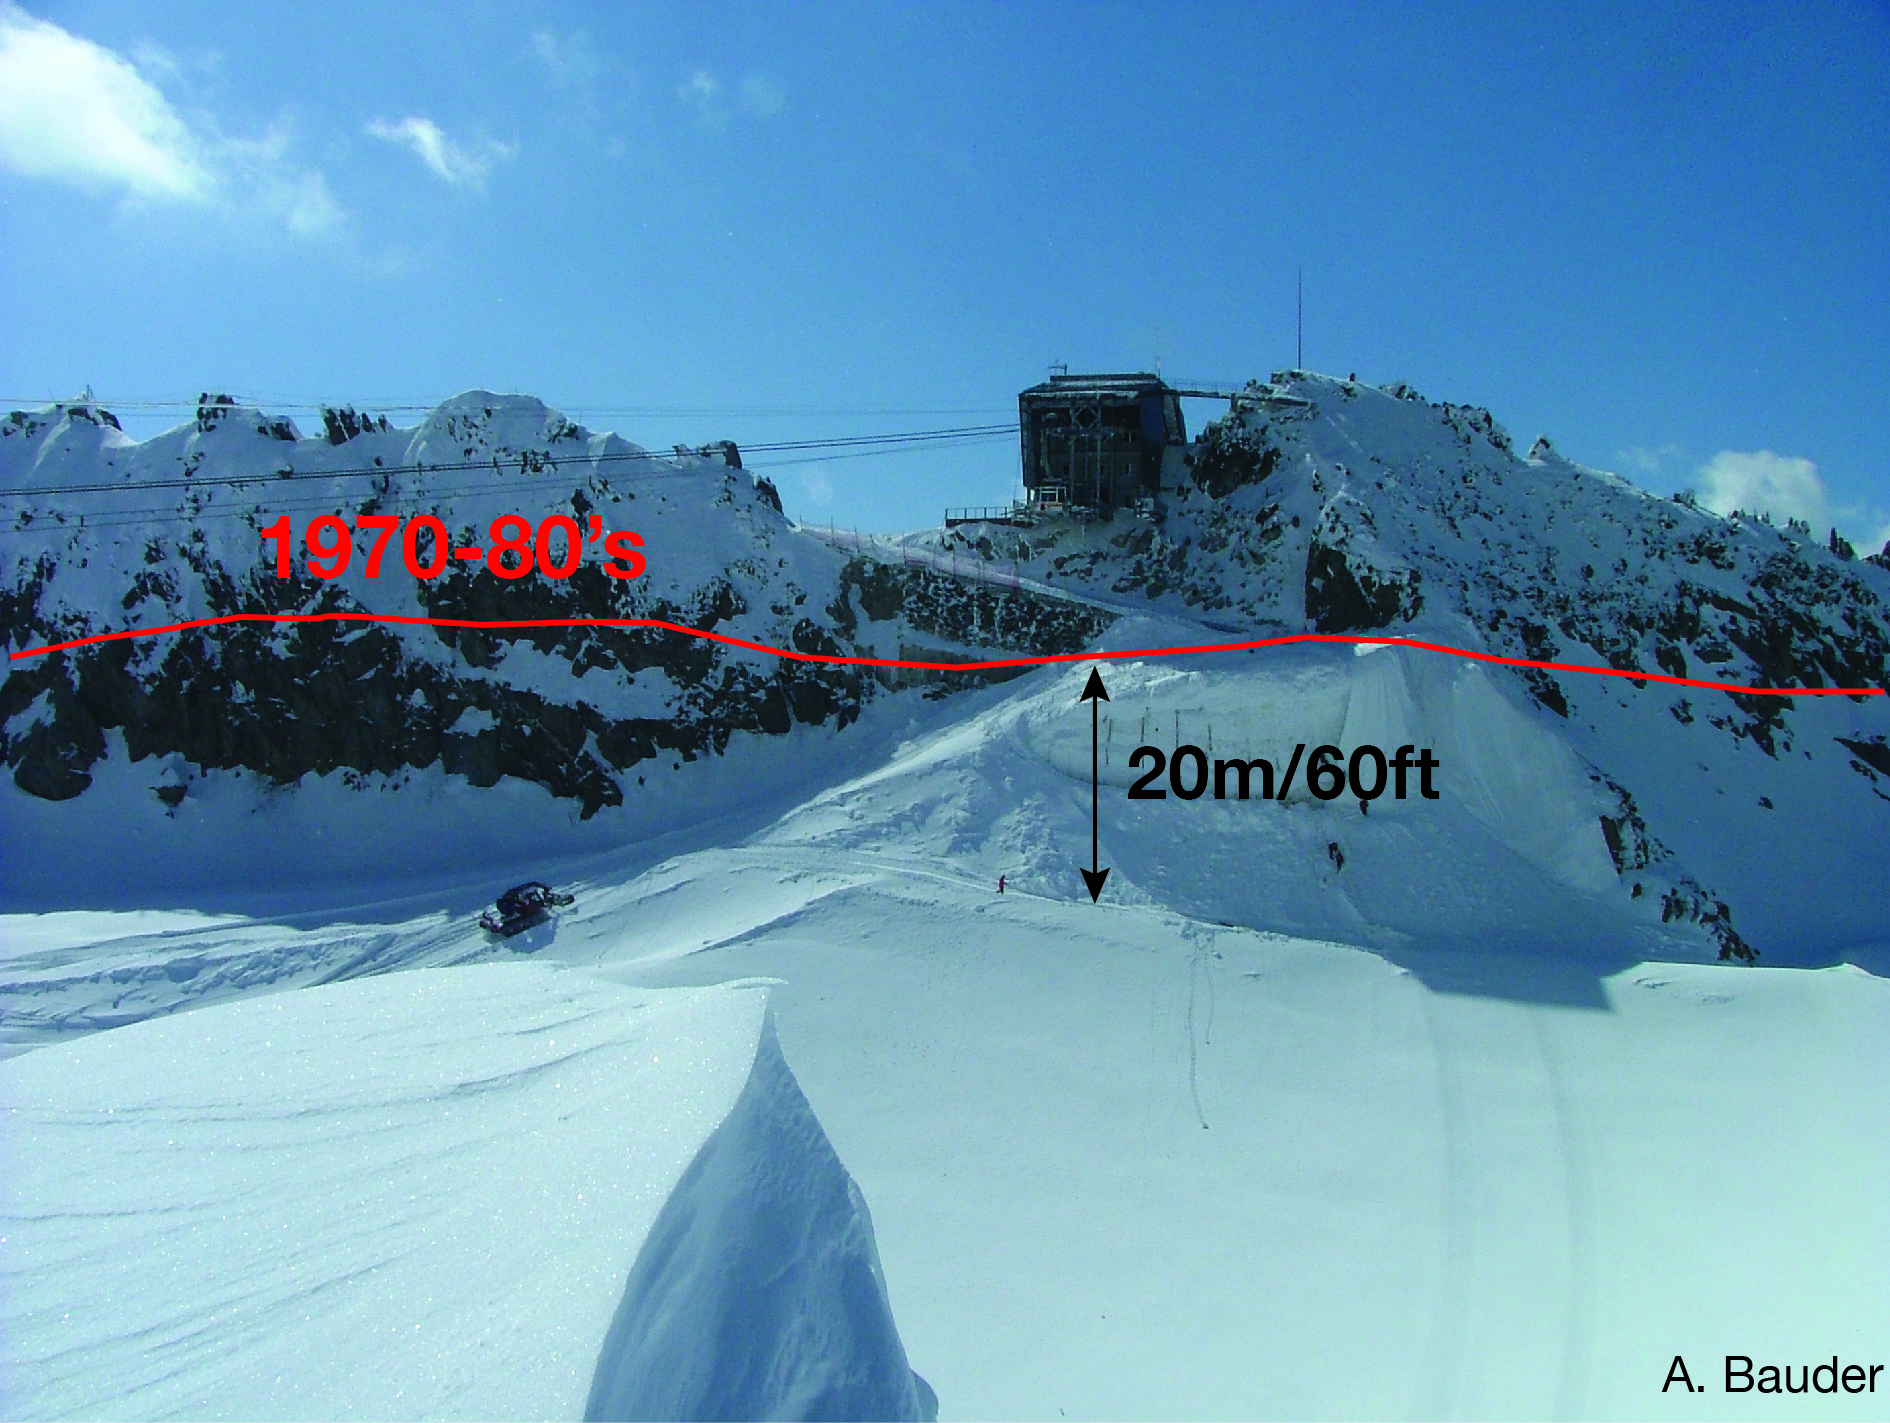
\includegraphics[width=\paperwidth]{gurschen-bauder}};}
}


\begin{frame}[plain]
  \note[item]{For example, when I was little we got out of the gondola}
  \note[item]{and we started to ski right on the glacier}
  \note[item]{However, in the past 2 or 3 decades, the glacier thinned by 20\,m or more}
  \note[item]{To get skiers on the glacier, they have to build a ramp out of snow every year}
  \note[item]{This is quite labor intensive and requires a lot of gas}
  \note[item]{Now, every spring ski patrol covers the ramp with a white tarp to preserve as much as possible}
  \note[item]{for the next winter}
  \note[item]{But glaciers are not thinning only in Switzerland}
\end{frame}
  
  
\setbeamertemplate{background canvas}
{
} 


% \begin{frame}
%   \begin{itemize}
%     \item Presently, 10 percent of land area on Earth is covered with glacial ice, including glaciers, ice caps, and the ice sheets of Greenland and Antarctica. Glacierized areas cover over 15 million square kilometers (5.8 million square miles).
%     \item Glaciers store about 75 percent of the world's fresh water.
%     \item During the maximum point of the last ice age, glaciers covered about 32 percent of the total land area.
% \item size of AK: 663,268 sq mi (1,717,856 km2), glaciers: 87,000 sq km
%   \end{itemize}
% \end{frame}

% \begin{frame}
% \begin{itemize}
% \item what do we use glaciers for?
% \item contain 75\% of the world's fresh water
% \item electricity, hydrodam, summer
% \end{itemize}
% \end{frame}

% \begin{frame}{Glaciers Flow}
% \begin{itemize}
% \item what do we use glaciers for?
% \item contain 75\% of the world's fresh water
% \item electricity, hydrodam, summer
% \end{itemize}
% \end{frame}


% \begin{frame}{Witnessing Glacier Change in Switzerland}
%       \begin{figure}
%         \only<1>{1994\\}
%         \only<2>{2006\\}
%         \includegraphics<1>[width=\textwidth]{steigletscher-repeat-1994}
%         \includegraphics<2>[width=\textwidth]{steigletscher-repeat-2006} 
%         {\\ \footnotesize{www.swisseduc.ch}}
%       \end{figure}
% \end{frame}

\setbeamertemplate{background canvas}
{
  \tikz{\node[inner sep=0pt,opacity=0.5] {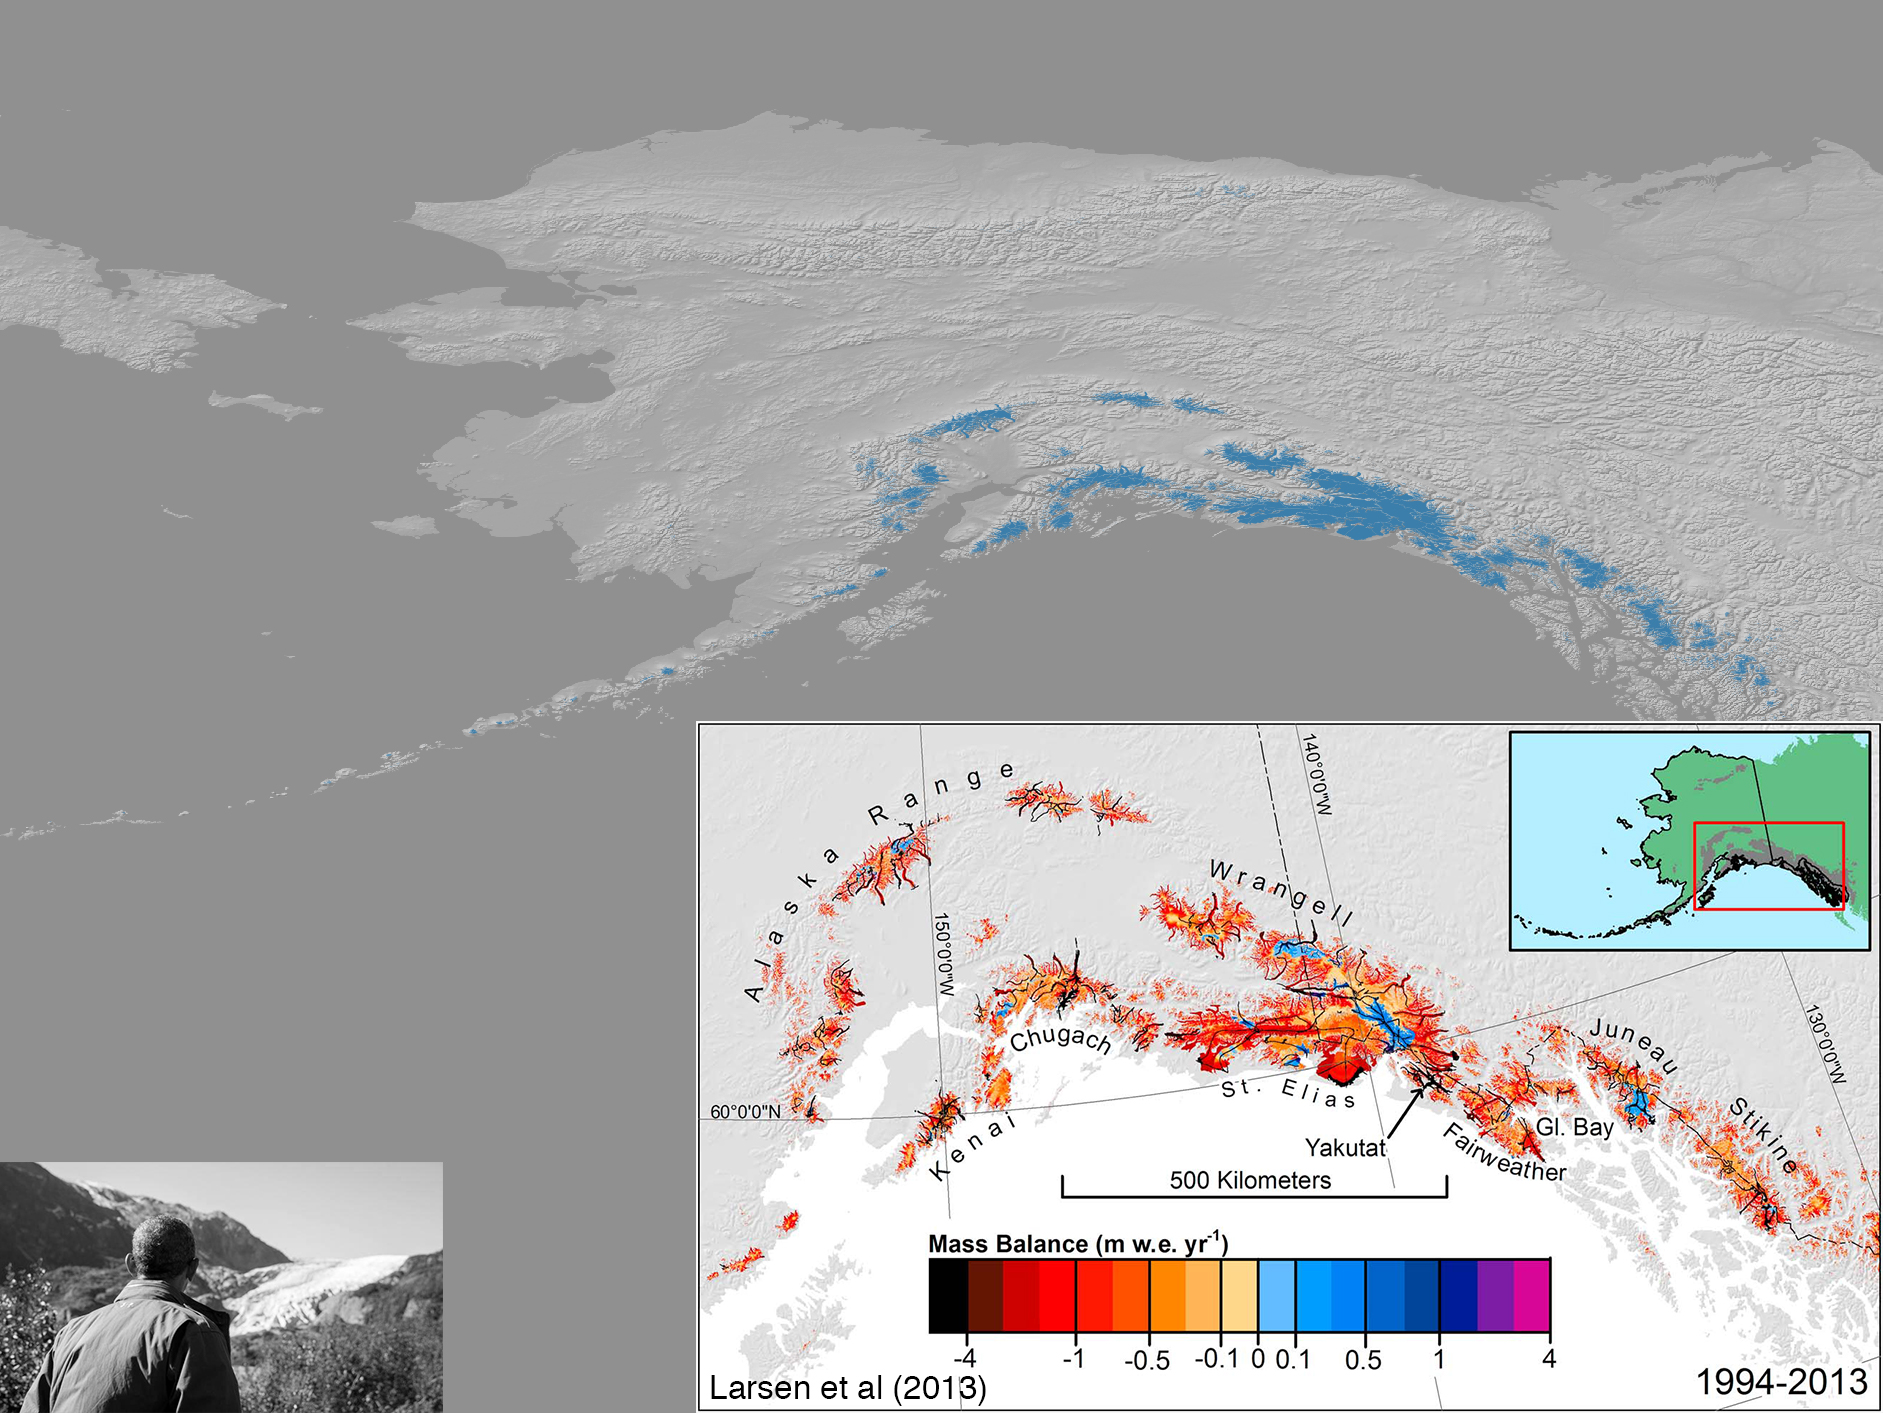
\includegraphics[width=\paperwidth]{ak_glacierized_area_16x12}};}
}



\begin{frame}{Melting Glaciers in Alaska: Columbia Glacier}
  \begin{figure}
    \movie[showcontrols=true,autostart,loop,width=12cm]{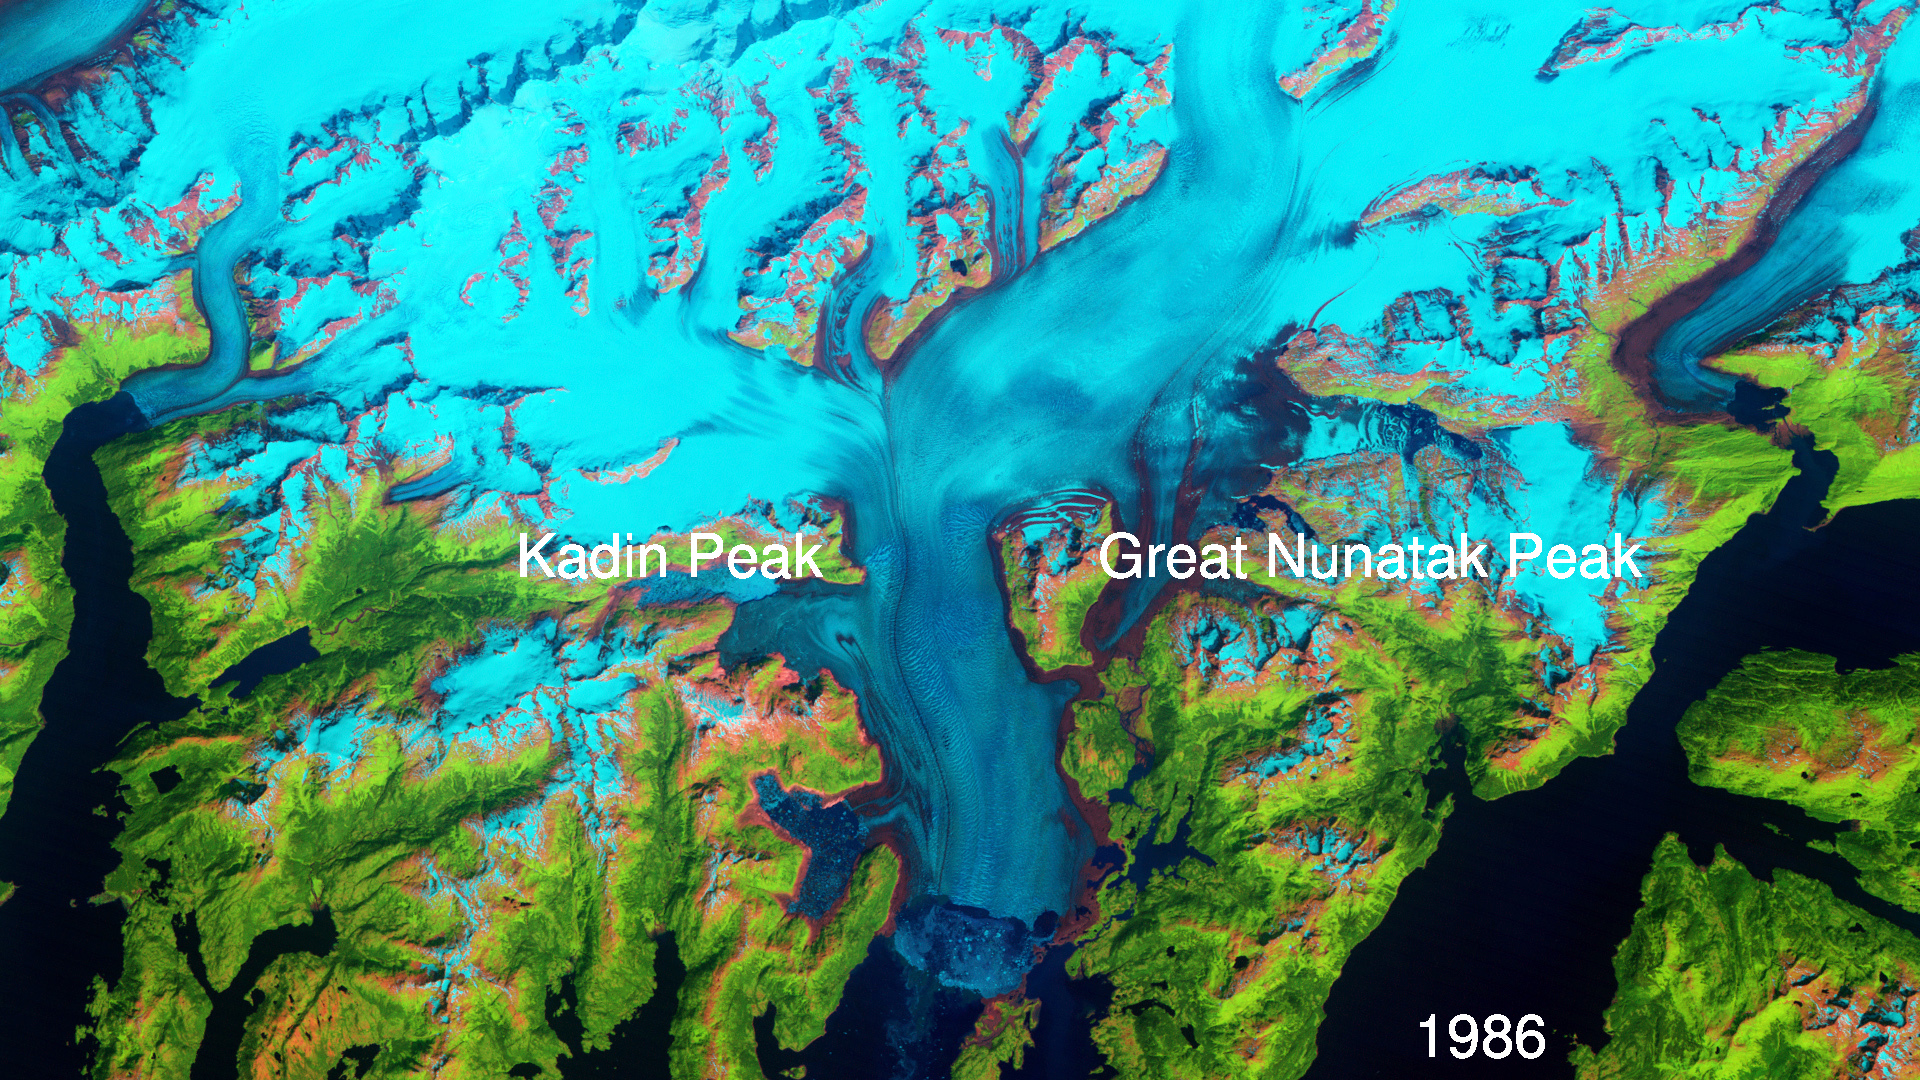
\includegraphics[width=12cm]{columbia_year_0000}}{columbia_landsat-hd1920.mov}
    {adapted from NASA's Scientific Visualization Studio}
  \end{figure}
  \note{In Alaska, they are changing too. Columbia glacier for example.}
  \note{Who has been to Columbia Glacier near Valdez?}
  \note{When British explorers first surveyed it in 1794, its terminus extended south to the northern edge of Heather Island, a small island. The glacier held that position until 1980, when it began a rapid retreat that continues today.}
\note{These false-color images, captured by Landsat satellites, show how the glacier and the surrounding landscape has changed since 1986.}
\note{Over the past three decades, the terminus had retreated more than 20 kilometers (12 miles). In some years, the terminus retreated more than a kilometer. Between 2000 and 2006 retreat stalled because the Great Nunatak Peak and Kadin Peak (directly to the west) constricted the glacier's movement and held the ice in place.}
\note{Between 2007 and 2010, part of the terminus began to float as it passed through deep water between the Great Nunatak Peak and Kadin Peak. This changed the way icebergs calved significantly. When the Columbia was grounded, calving occurred at a fairly steady rate, and the bergs that broke off were small. When the glacier began to float, larger chunks of ice tended to break off, as seen in the image from 2009.}
\end{frame}


% \begin{frame}{Glacier Change in Alaska: Columbia Glacier}
%   \movie[showcontrols=true,autostart,loop,width=12cm]{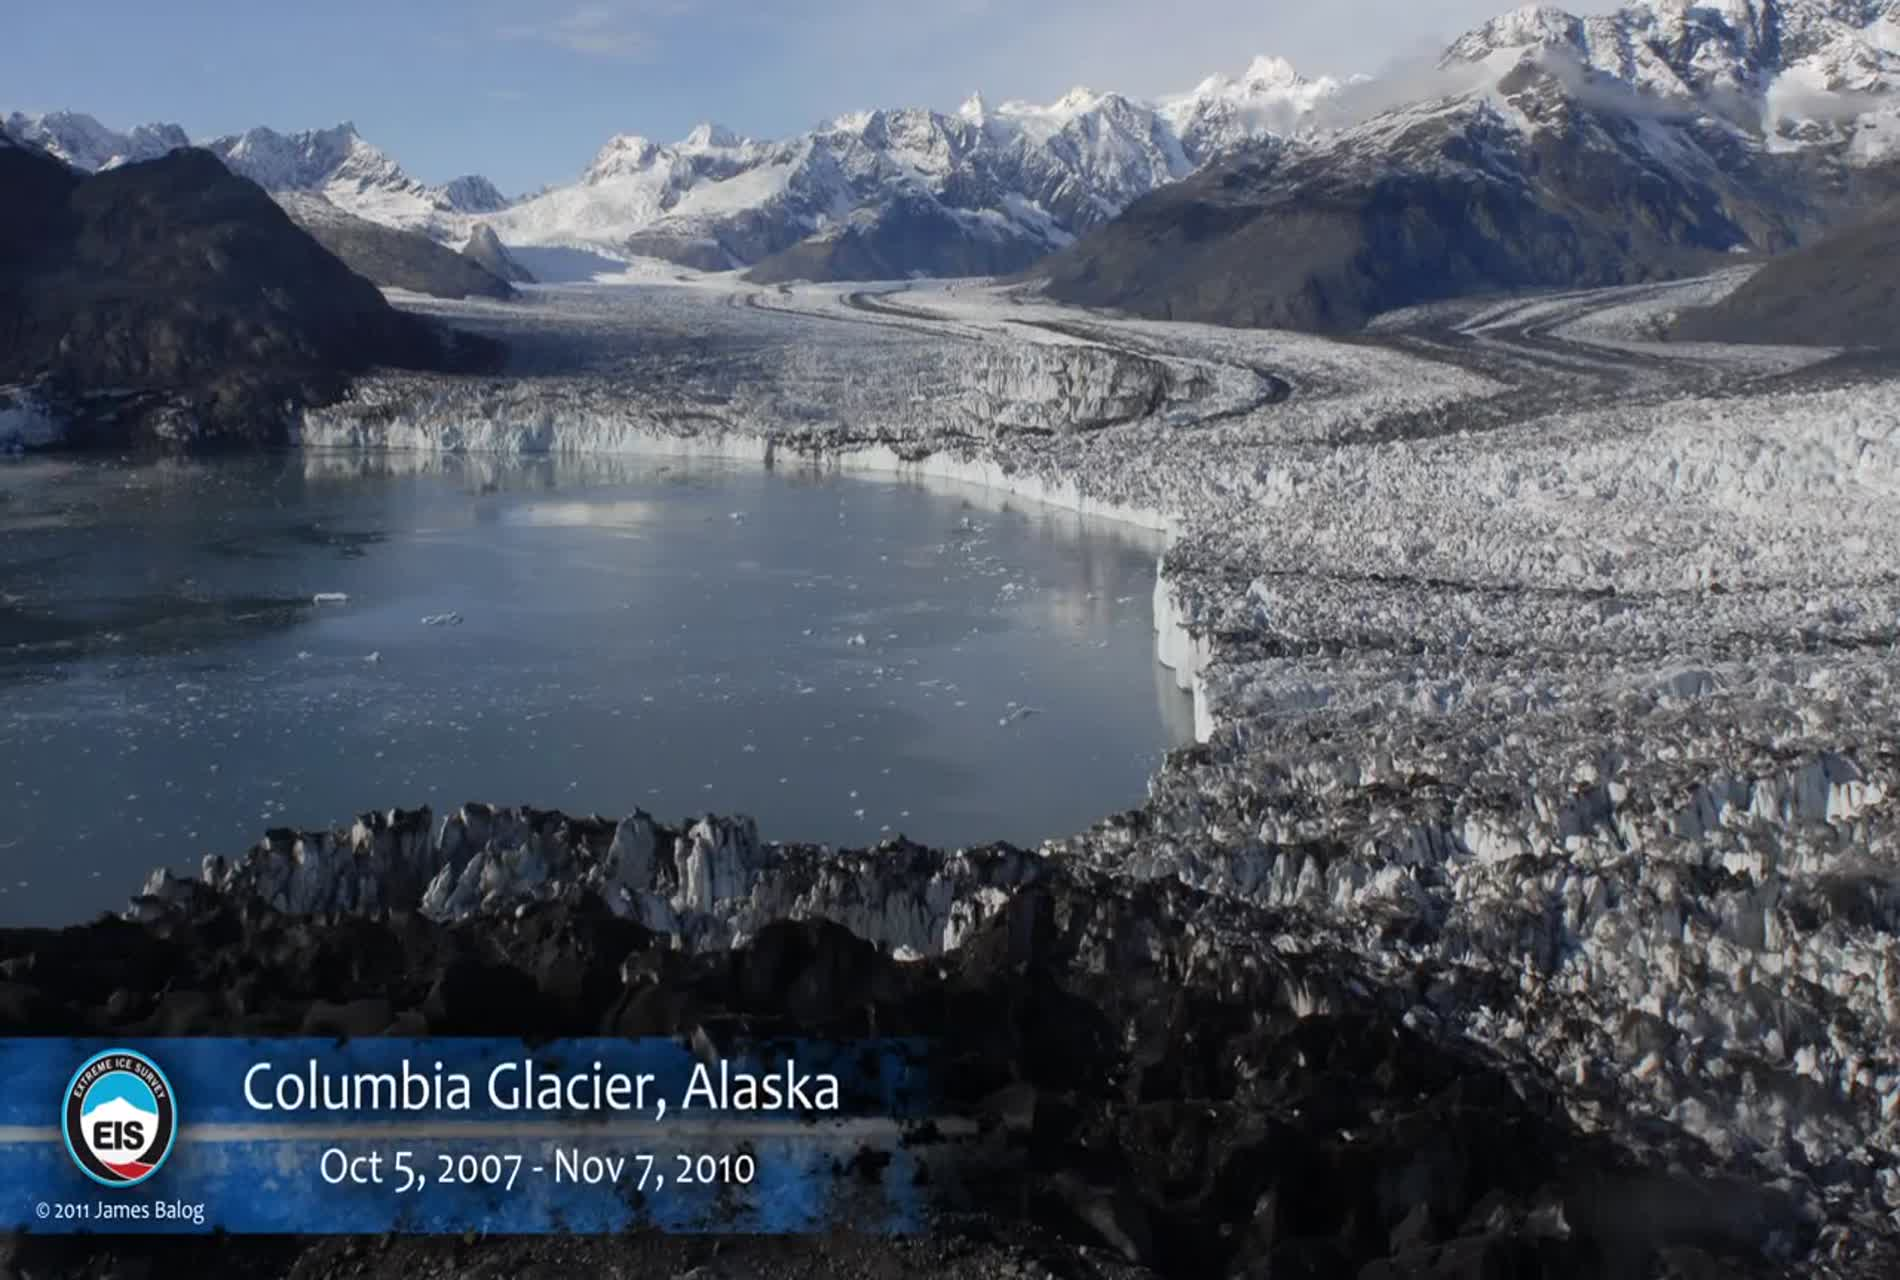
\includegraphics[width=12cm]{columbia-eis}}{columbia-eis.mov}
% \end{frame}


\setbeamertemplate{background canvas}
{
  \tikz{\node[inner sep=0pt,opacity=0.75] {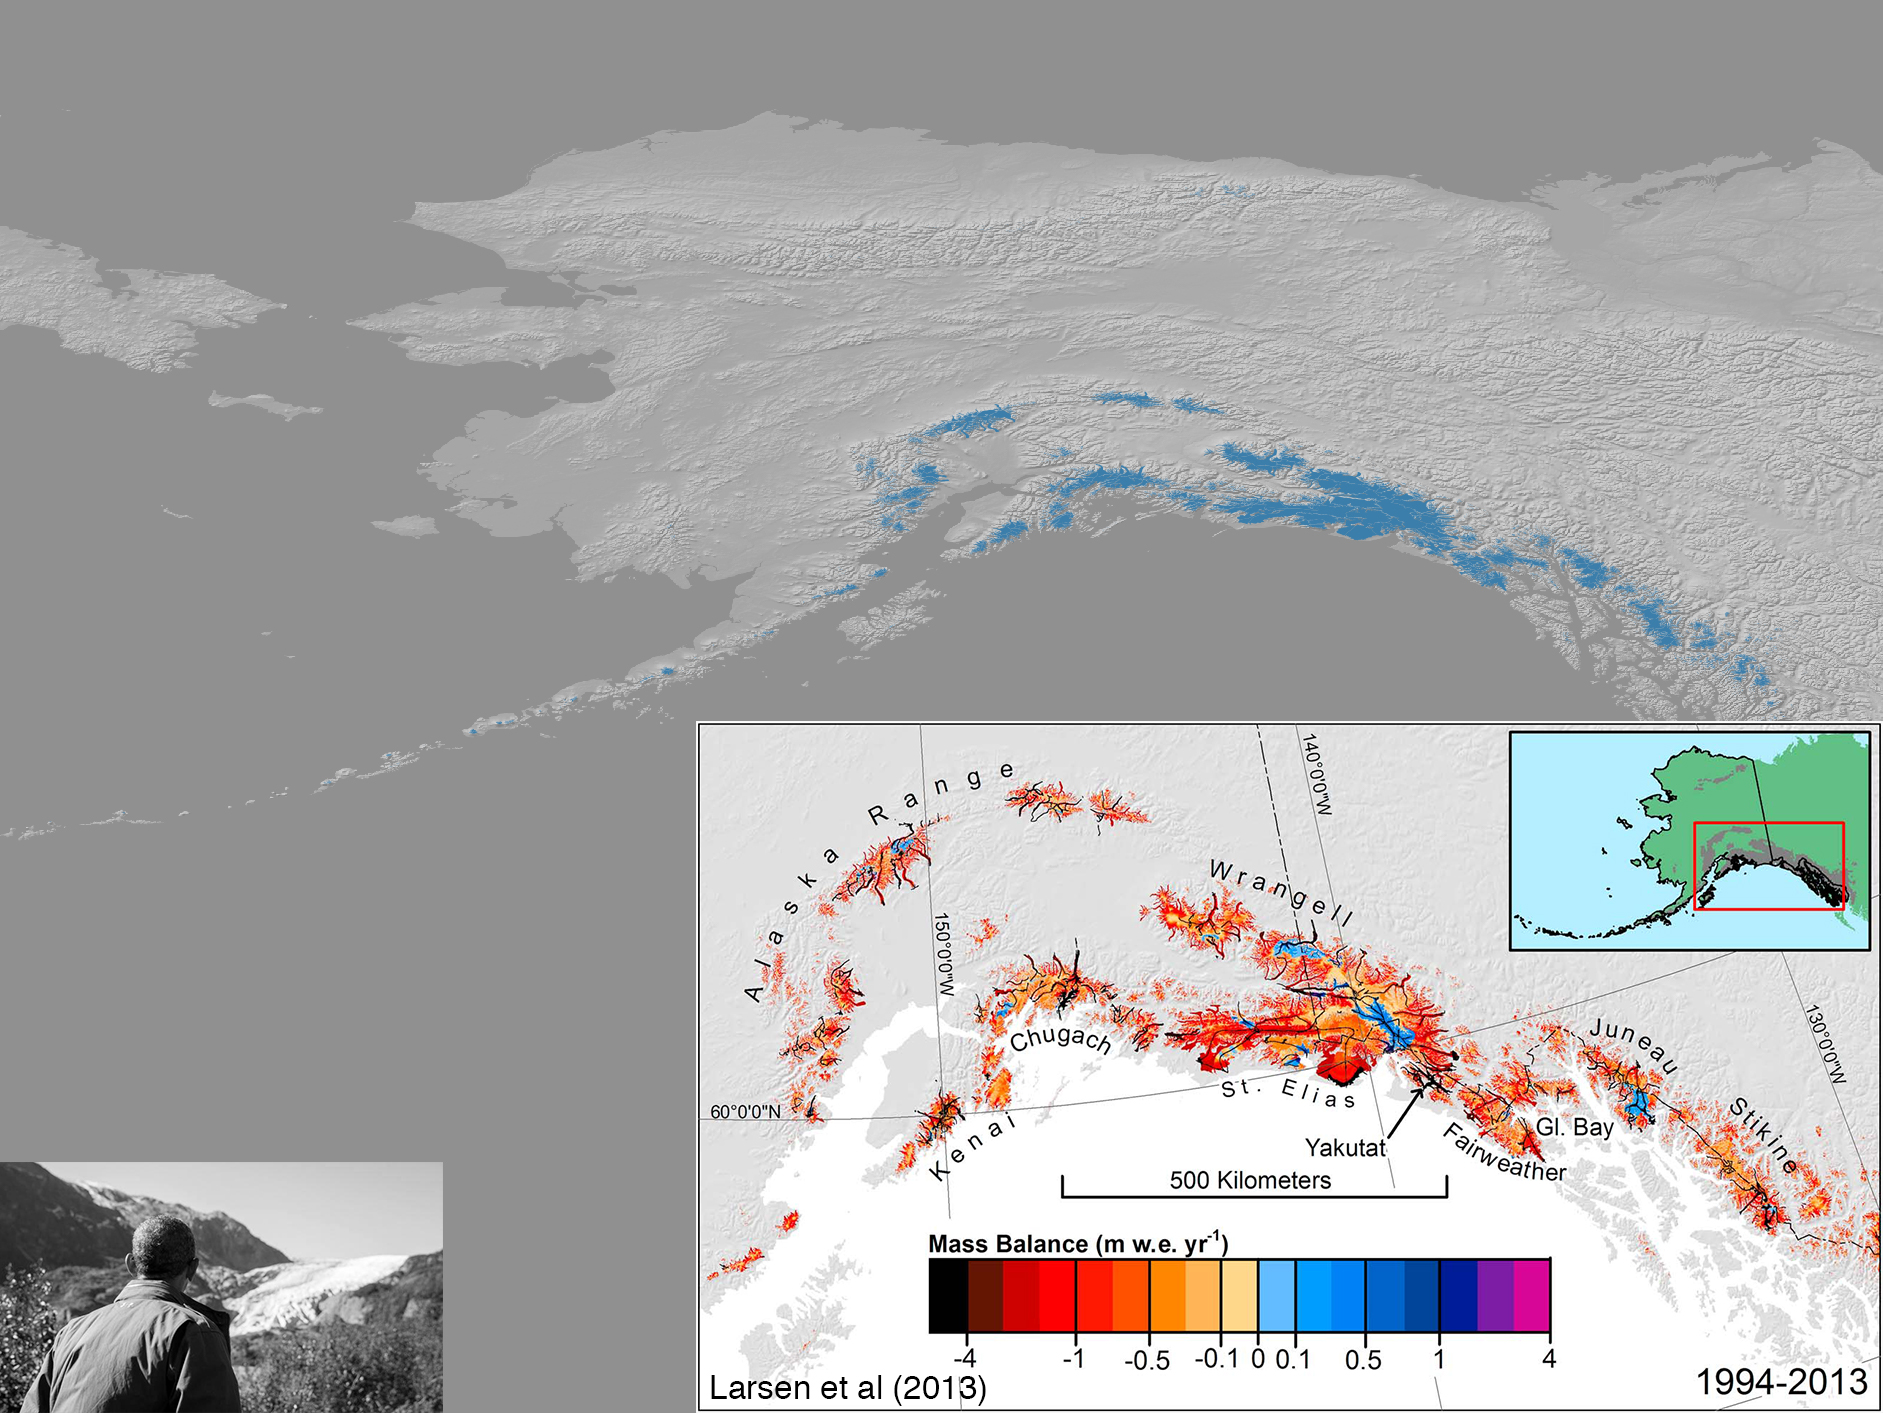
\includegraphics[width=\paperwidth]{ak_glacierized_area_melt_16x12}};}
}

\begin{frame}{Melting Glaciers in Alaska}
  \begin{itemize}
  \item total mass loss 1994--2013 from AK glaciers: 75$\pm$11 Gt/yr loss $\Rightarrow$ 5\,cm (1.5\,in) layer of water covering Alaska
  \end{itemize}
  \note[item]{Columbia Glacier is not alone}
  \note[item]{How many glaciers are losing mass}
\end{frame}

\setbeamertemplate{background canvas}
{
}


% \setbeamertemplate{background canvas}
% {
%   \tikz{\node[inner sep=0pt,opacity=0.75] {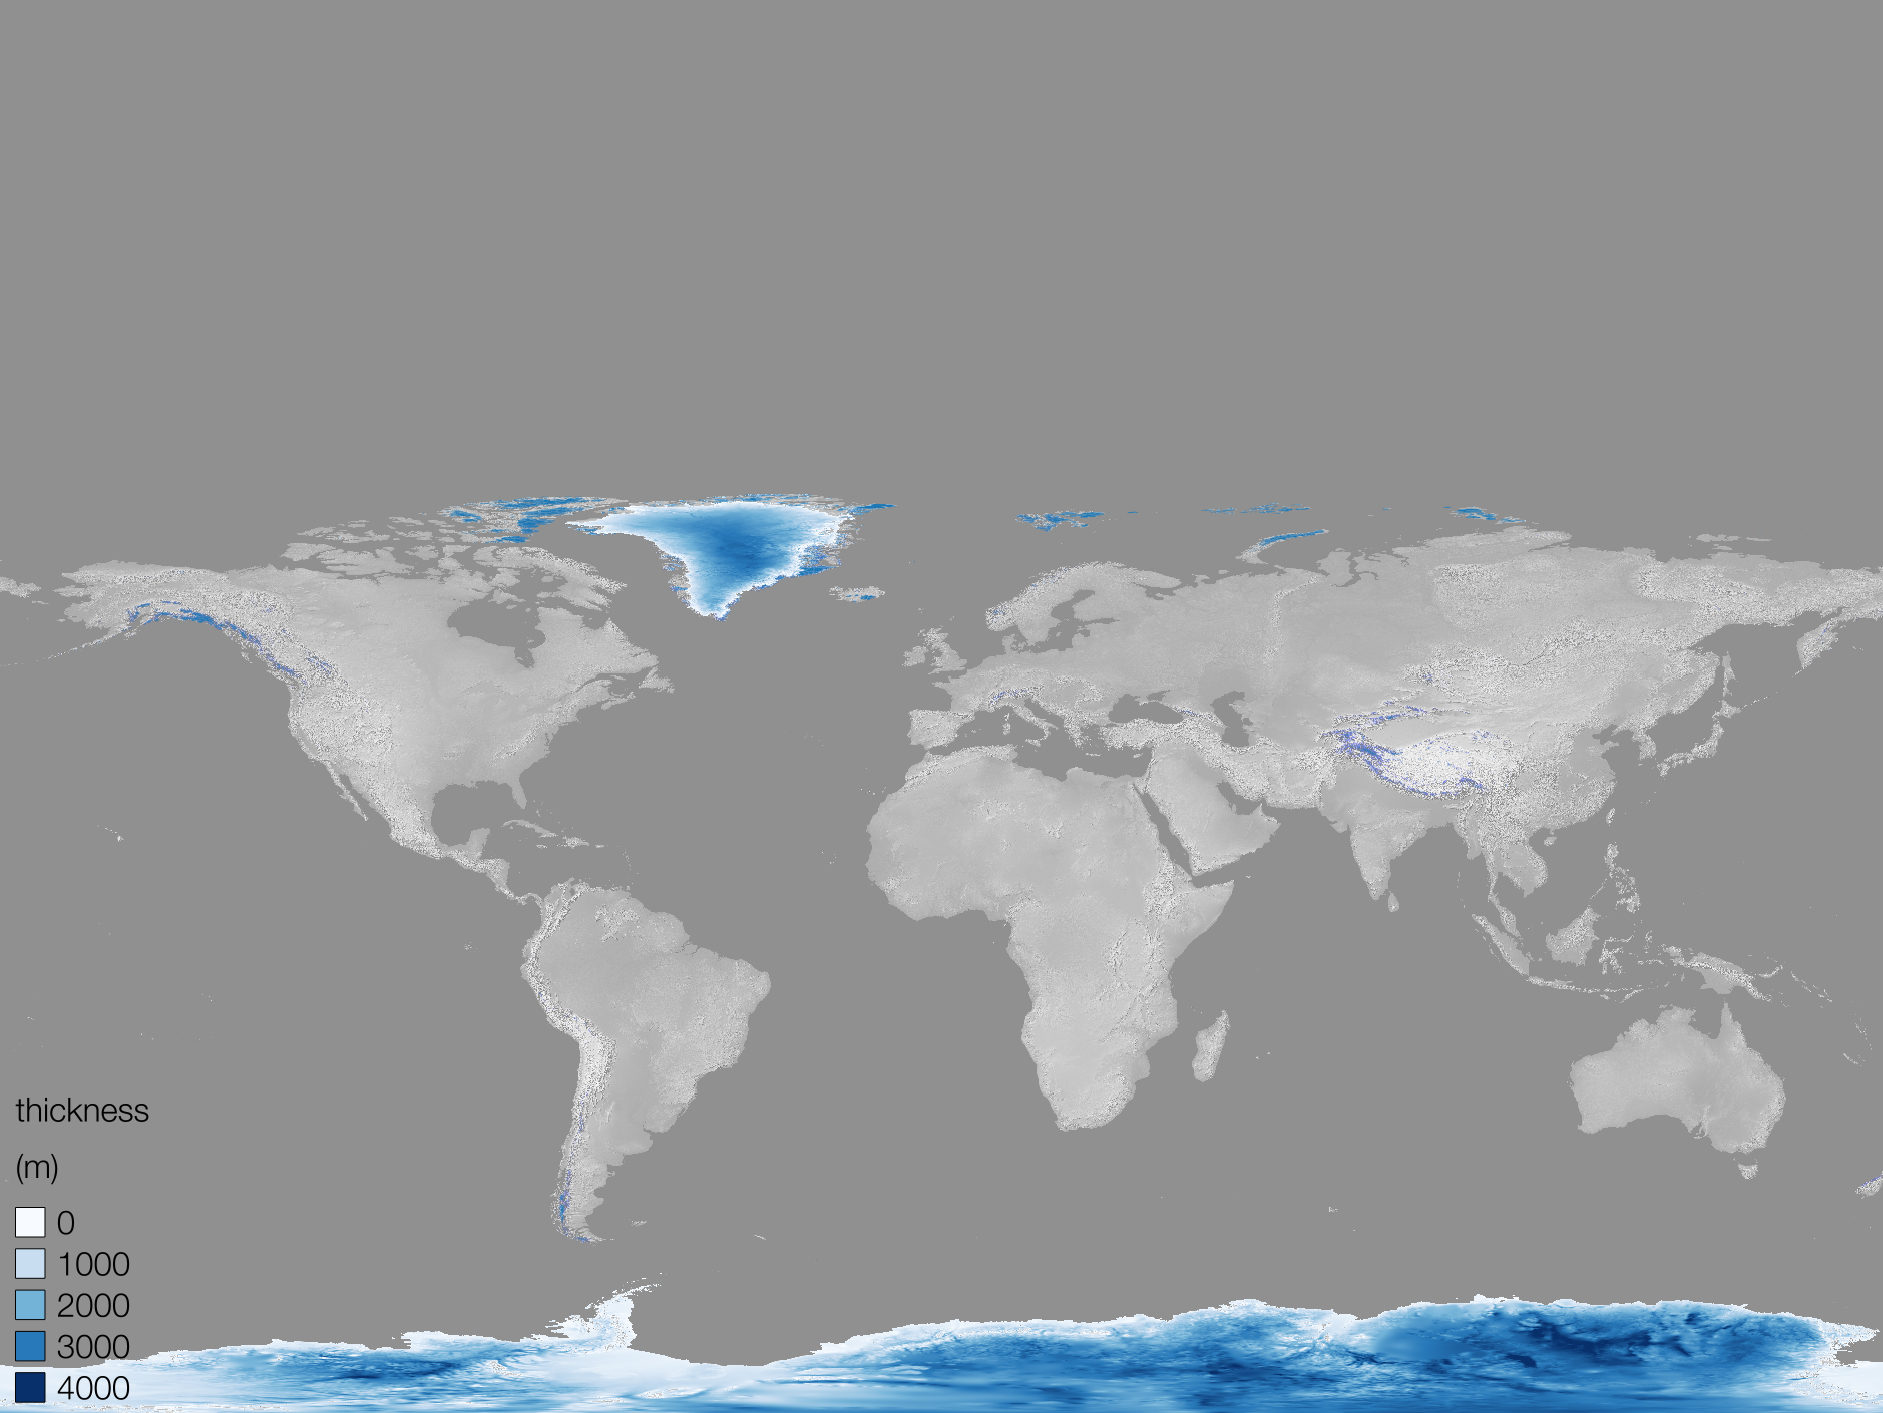
\includegraphics[width=\paperwidth]{world_glacierized_area_16x12}};}
% }

% \begin{frame}{Glacier Change Worldwide}
%   \begin{itemize}
%     \item Presently, 10\,\% of land area is covered with ice
%     \item That's about 10 times the size of Alaska
%   \end{itemize}
% \end{frame}


% \setbeamertemplate{background canvas}
% {
% }

\begin{frame}{Melting Glaciers Everywhere: The Biggest Losers}
  \begin{figure}
    {Alaska \qquad---\qquad West Greenland \qquad---\qquad West Anartica}
    \\[1em]
    \includegraphics<1>[width=1\textwidth]{grace-world-2003-2010-01}
  \end{figure}
\end{frame}

\begin{frame}{Glacier and Climate}
But glaciers and the climate are constantly changing, right

Look at the past
\end{frame}



\begin{frame}{The sun drives the glacial/interglacial cycle}
  \vspace{-2cm}
  \begin{block}{Milankovitch Cycle}
    \begin{figure}
      \movie[showcontrols=true,autostart,loop,width=8cm]{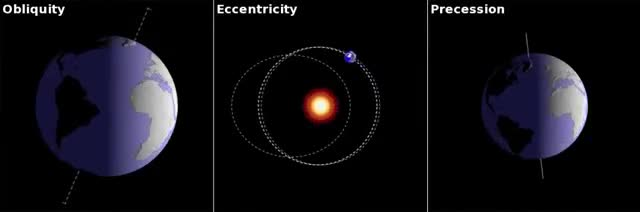
\includegraphics[width=8cm]{orbital-forcing}}{orbital-forcing.mov}
    \end{figure}
  \end{block}
  \begin{columns}[T]
    \begin{column}{.32\linewidth}
      41,000 yrs
    \end{column}
    \begin{column}{.32\linewidth}
      100,000 yrs
    \end{column}
    \begin{column}{.32\linewidth}
      26,000 yrs
    \end{column}
  \end{columns}
  \note[item]{Changes in the obliquity (tilt) of Earth's axis}
  \note[item]{Variations in the shape of Earth's orbit (eccentricity)}
  \note[item]{Changes in Earth's "Wobble" (Precession)}
\end{frame}


\begin{frame}
    \begin{figure}
      \movie[showcontrols=true,loop,width=10cm]{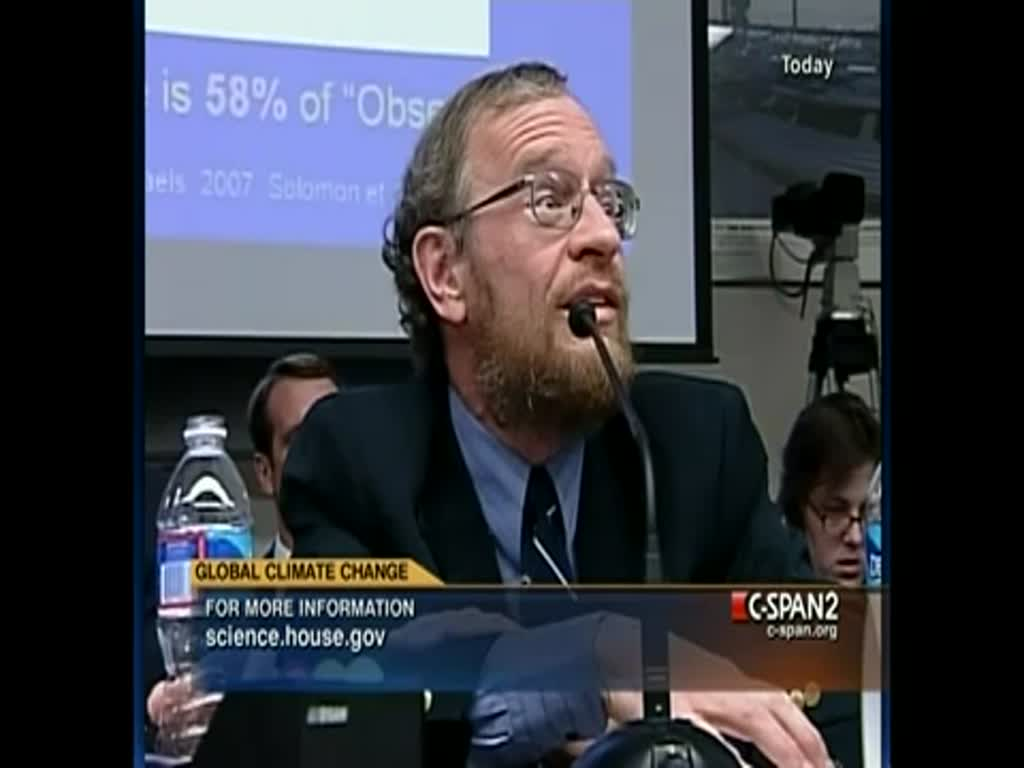
\includegraphics[width=10cm]{alley-001}}{alley-milankovitch.mov}
    \end{figure}
    \centering{CO$_2$ feedback needed}
    \note[item]{My colleague Richard Alley is much more eqloquent in explain what causes ice ages}
    \note[item]{as he did in this hearing in front of congress a couple of years ago}
\end{frame}

\setbeamertemplate{background canvas}
{
  \tikz{\node[inner sep=0pt,opacity=0.5] {
\includegraphics[height=\paperheight,width=\paperwidth]{ice-age}};}
}

\begin{frame}{Ice Ages}
  \vspace{1.5cm}
  \begin{figure}
    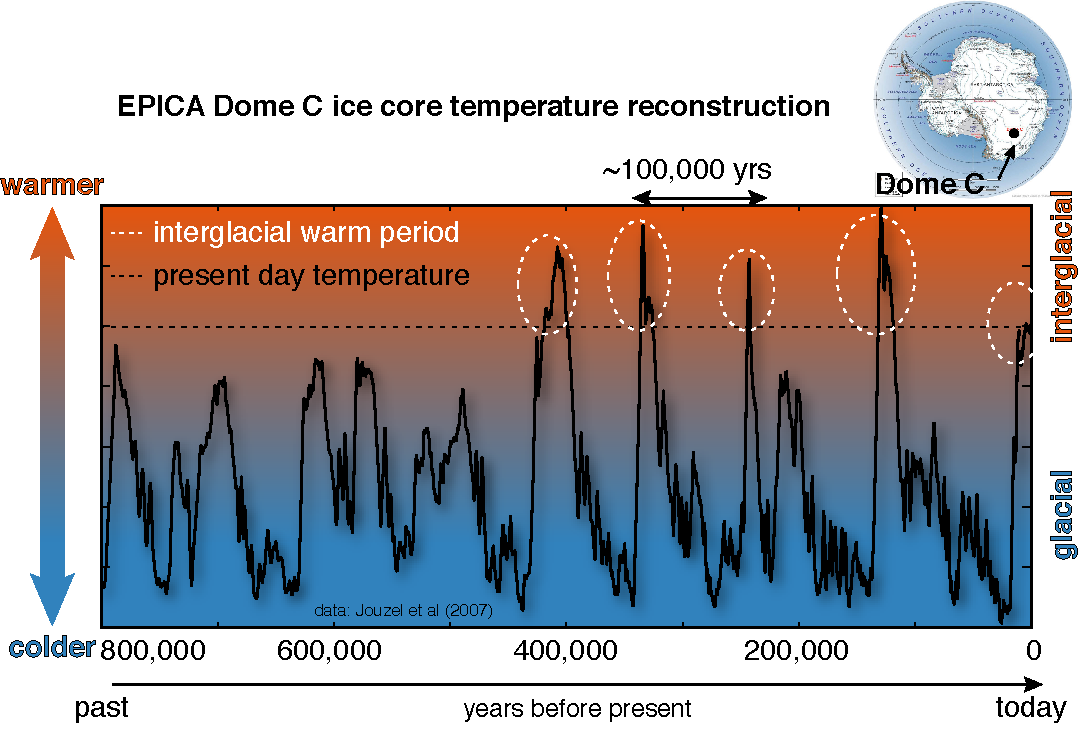
\includegraphics[width=\textwidth]{epica-temp}
  \end{figure}
\end{frame}

\setbeamertemplate{background canvas}
{
}



\begin{frame}{What if they melted completely?}
  \begin{figure}
    \includegraphics<1>[width=\textwidth]{sea-level-potential-simple-01}
    \includegraphics<2>[width=\textwidth]{sea-level-potential-01}
  \end{figure}
\end{frame}
  

\setbeamertemplate{background canvas}
  {
     \tikz{\node[inner sep=0pt,opacity=0.5] {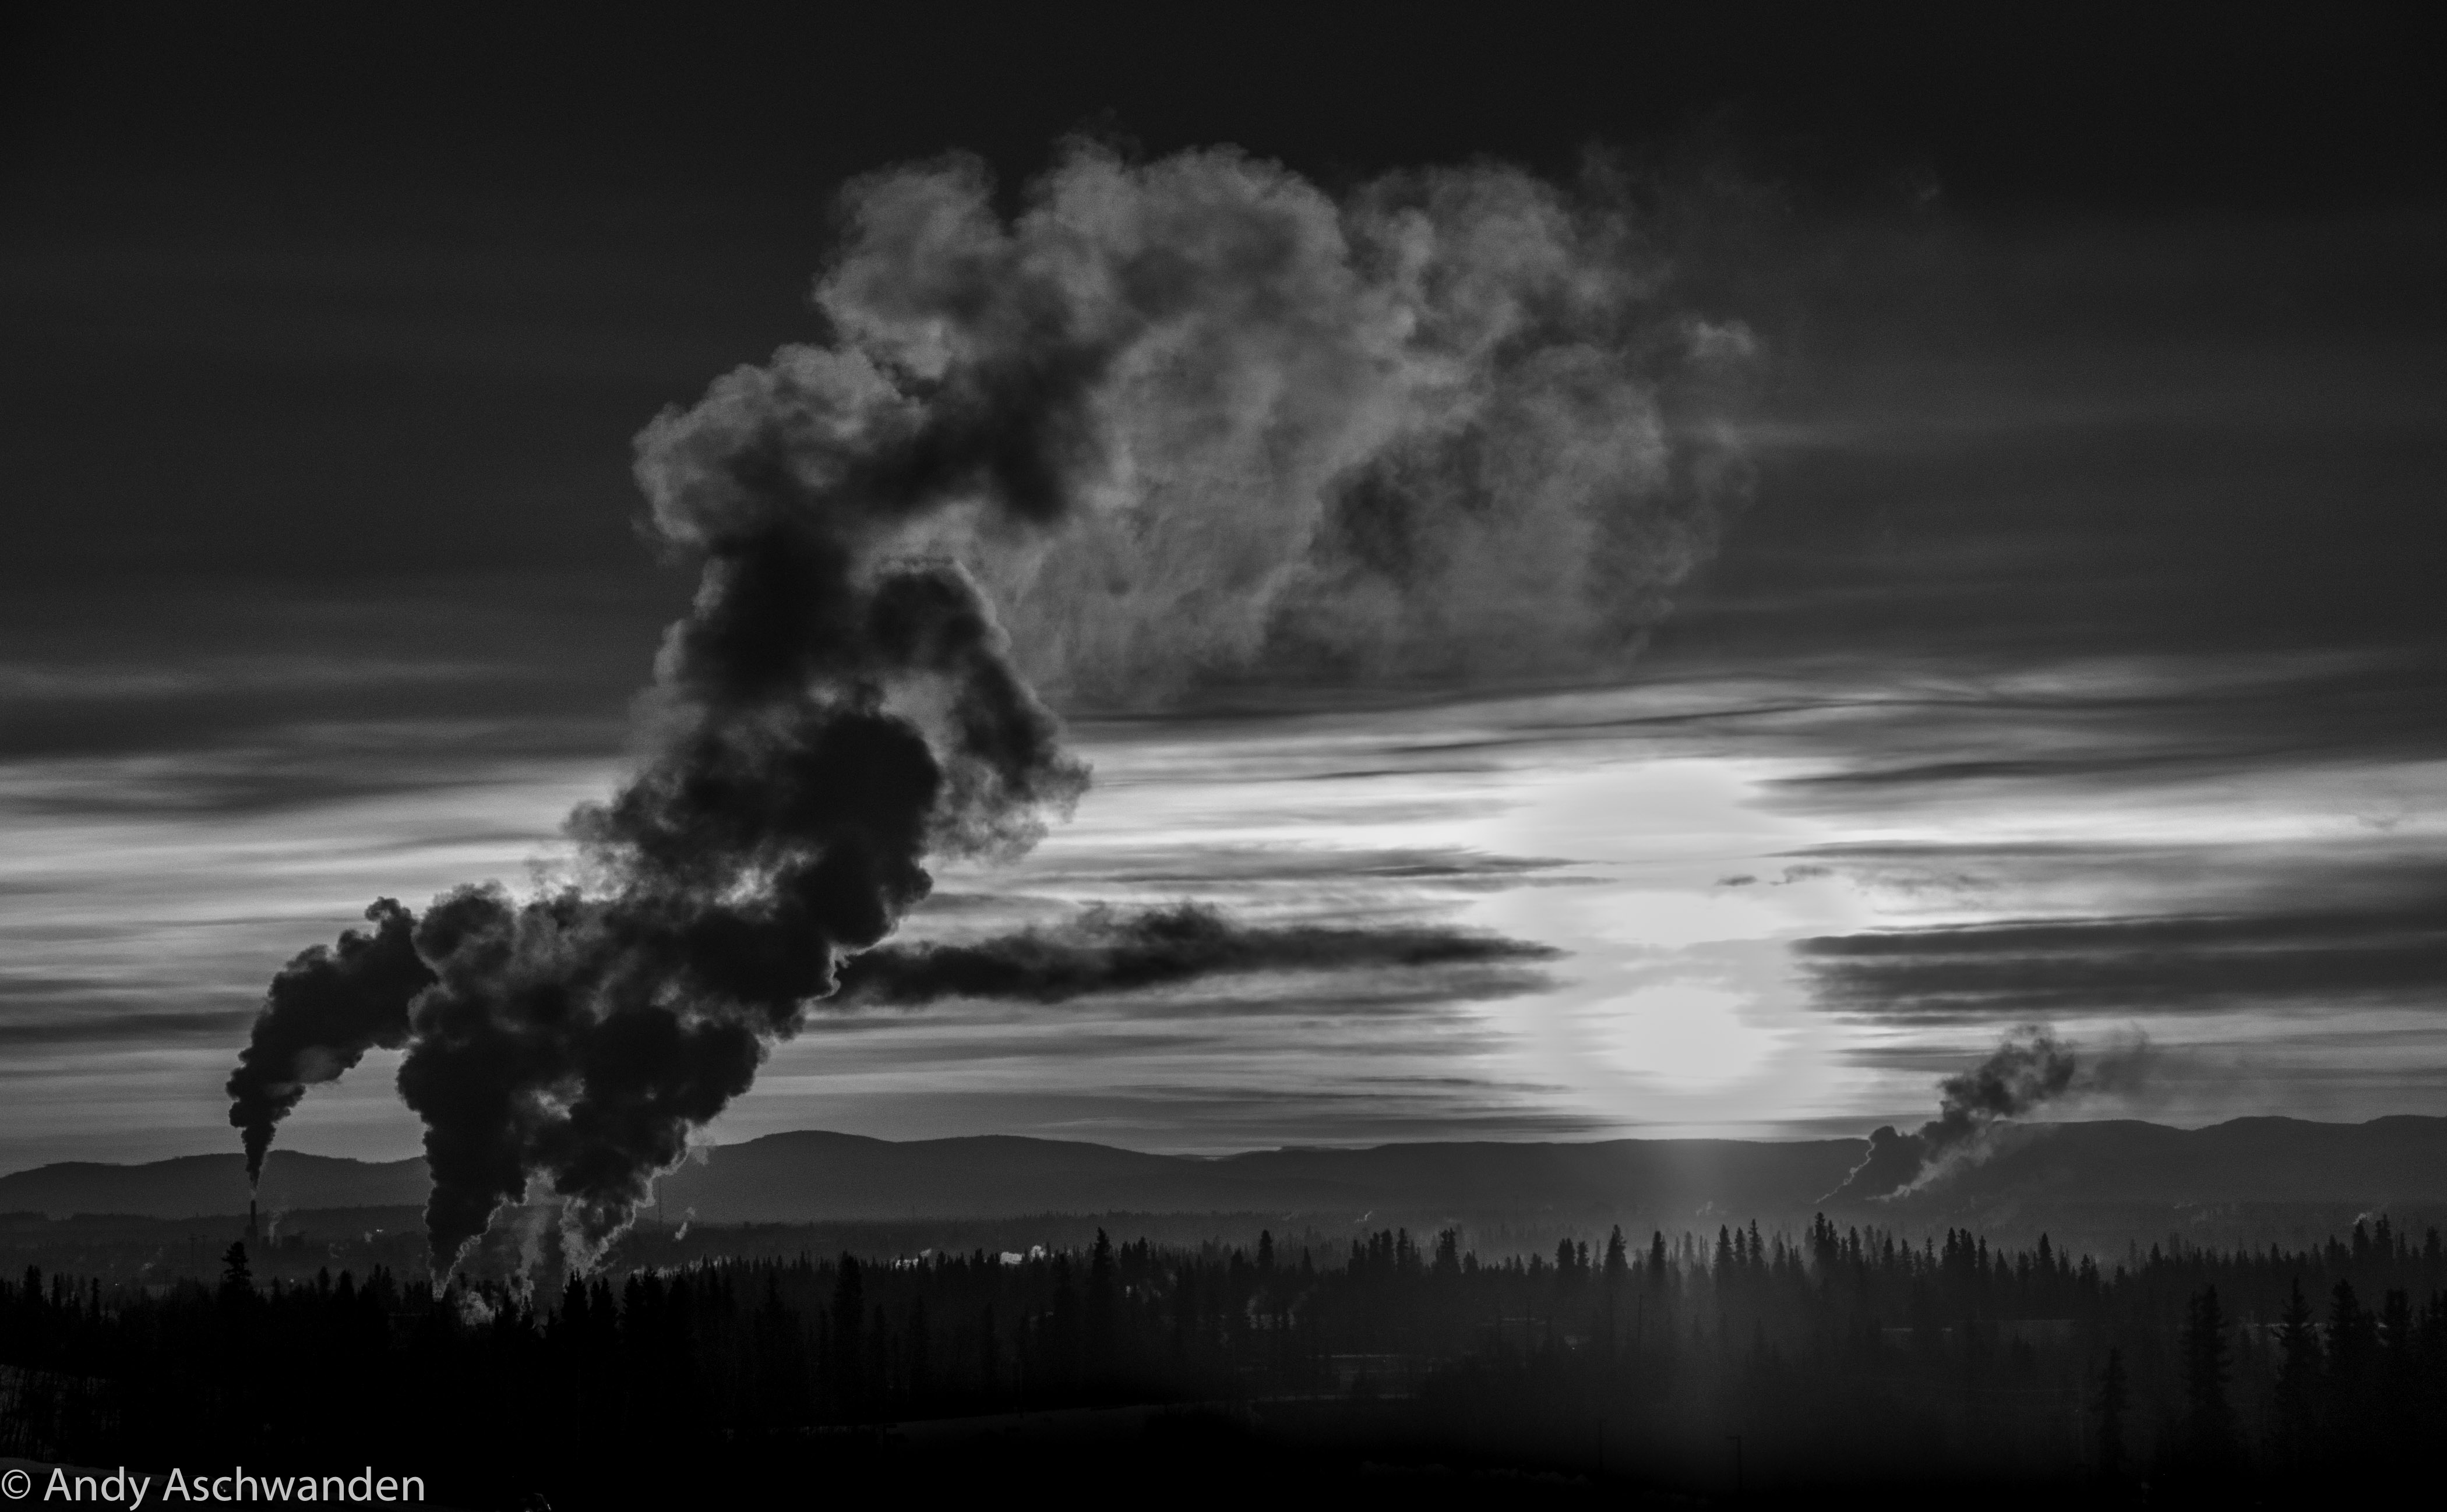
\includegraphics[height=\paperheight,width=\paperwidth]{uaf_power_plant}};}
} 

\begin{frame}{Could this happen?}
    \begin{itemize}
      \item Combustion of available fossil fuel resources sufficient to eliminate the Antarctic Ice Sheet (Winkelmann \emph{et al.}, 2015)
      \item and probably the  Greenland Ice Sheet too
    \end{itemize}
  \note[item]{My colleagues asked the question what would happen if\ldots}
\end{frame}


\setbeamertemplate{background canvas}
  {
     \tikz{\node[inner sep=0pt,opacity=1] {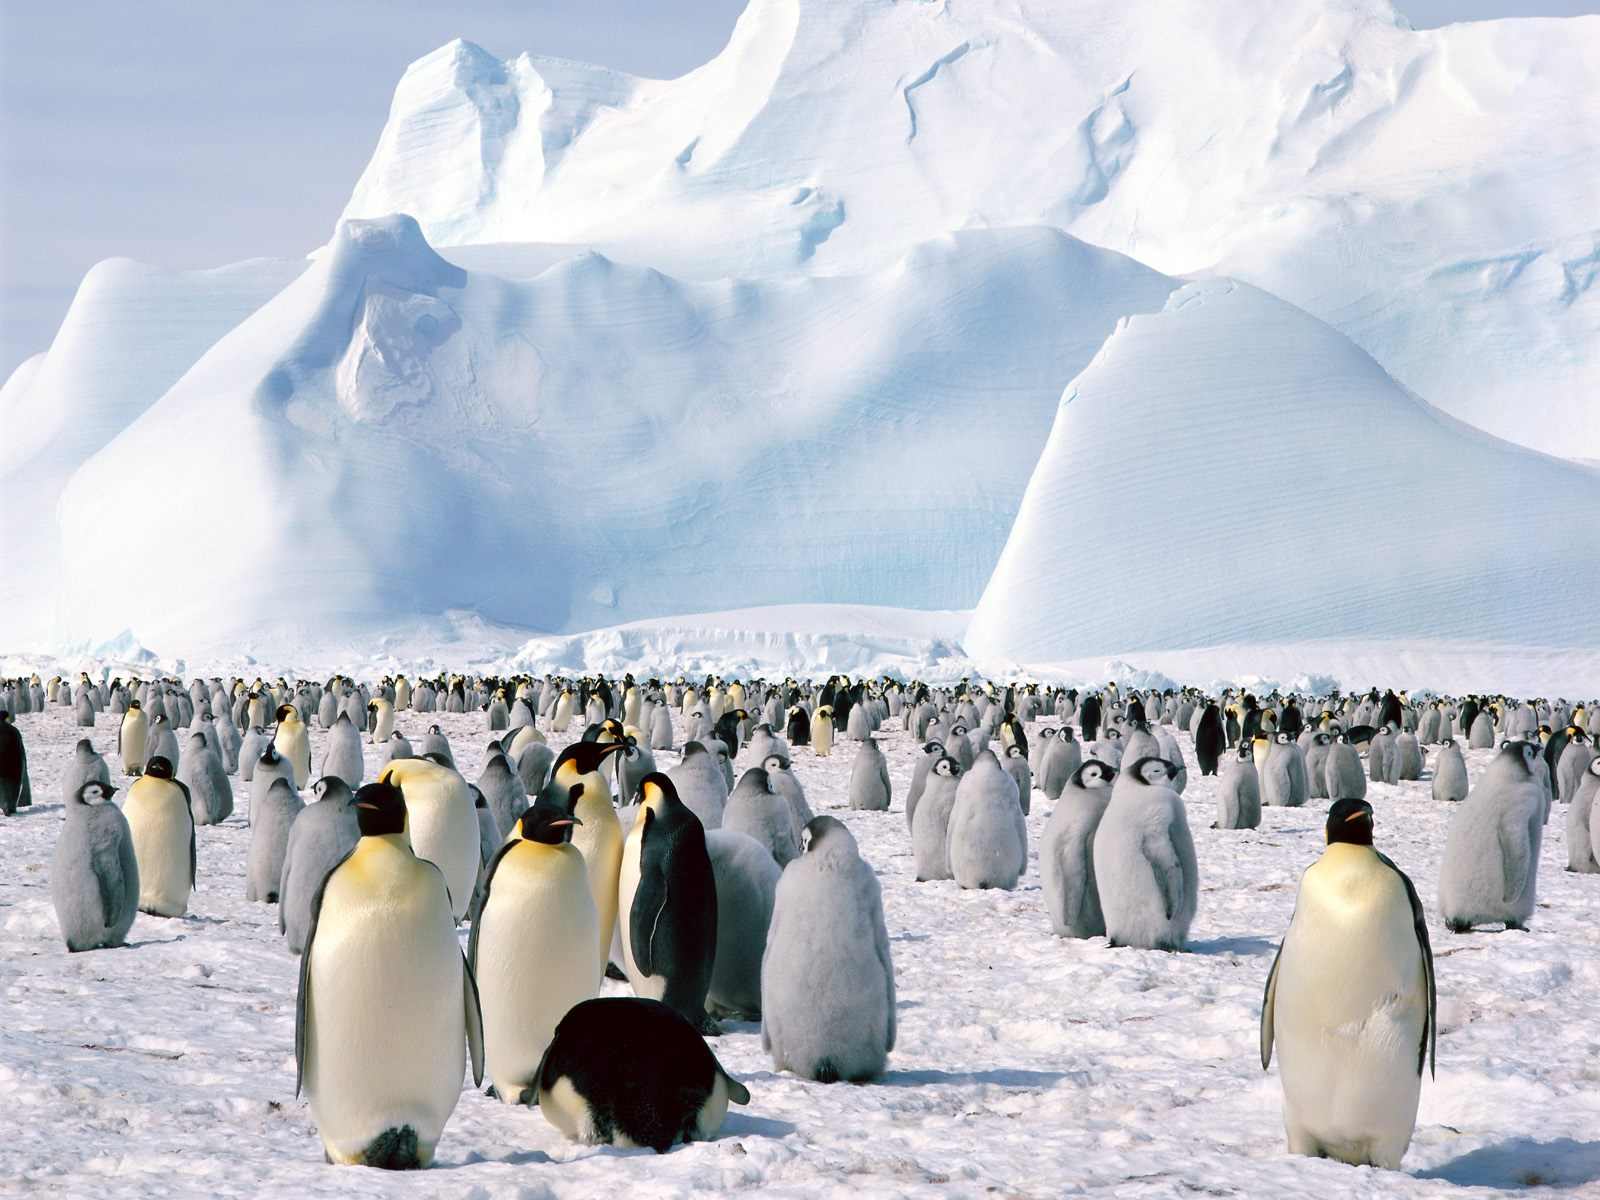
\includegraphics[height=\paperheight,width=\paperwidth]{ant_penguins}};}
} 

\begin{frame}[plain]
\end{frame}

\setbeamertemplate{background canvas}
  {
     \tikz{\node[inner sep=0pt,opacity=1] {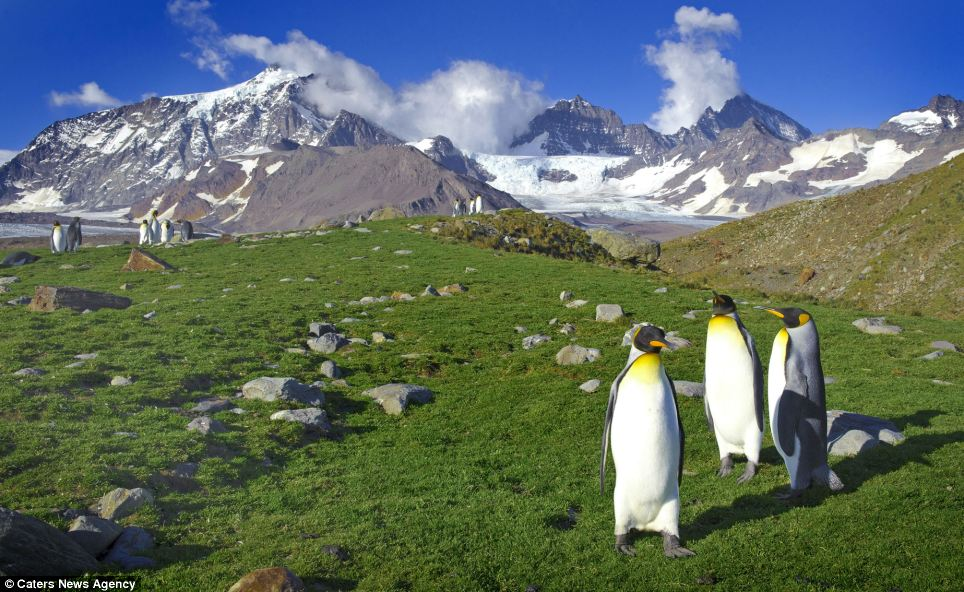
\includegraphics[height=\paperheight,width=\paperwidth]{green_penguins}};}
} 

\begin{frame}[plain]
\end{frame}

  
\setbeamertemplate{background canvas}
{
} 

\begin{frame}{??? What are the chances?}
\begin{itemize}
\item we need to understand how glaciers work
\end{itemize}
\end{frame}


\begin{frame}{How a glacier loses mass}
  \begin{figure}
    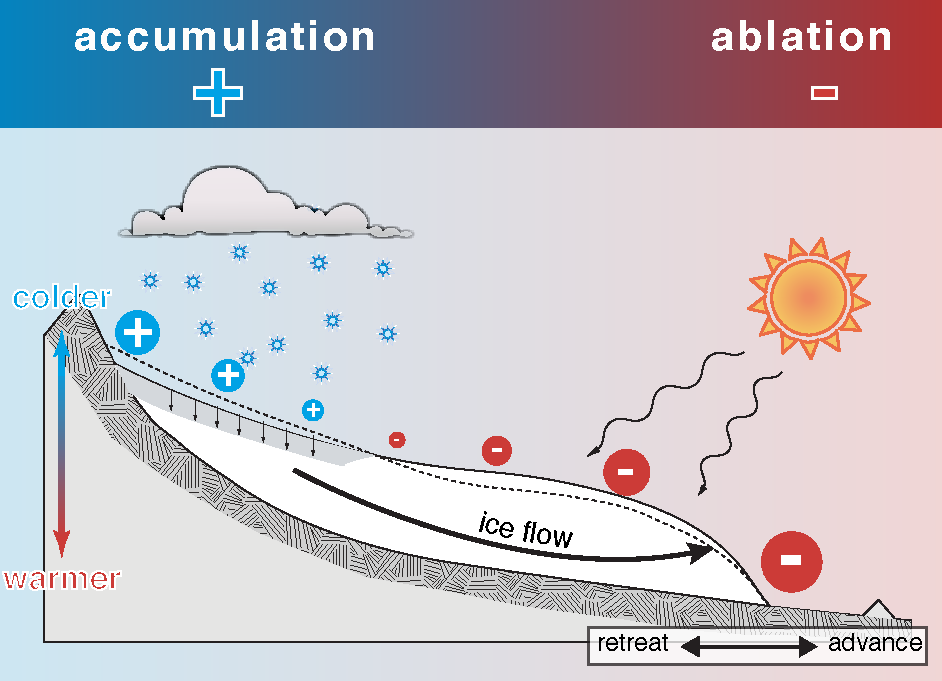
\includegraphics[width=\textwidth]{glacier_mb}
  \end{figure}
  \note[item]{in general, the higher up we go, the colder it gets}
  \note[item]{though this is not always true in Fairbanks}
  \note[item]{as those of you living up in the hills appreciate}
  \note[item]{and starts to flow downhill towards the coast}
  \note[item]{near the coast, surface melting can occur in the summer}
  \note[item]{but also some ice is dumped directly into the ocean}
  \note[item]{before the mid-90s mass loss was dominated by surface mass balance (80-90\%)}
  \note[item]{contribution of ice discharge was modest (10--20\%)}
  \note[item]{explaining in more detail in the next slide}
\end{frame}


\begin{frame}{How an ice sheet loses mass}
  \begin{figure}
    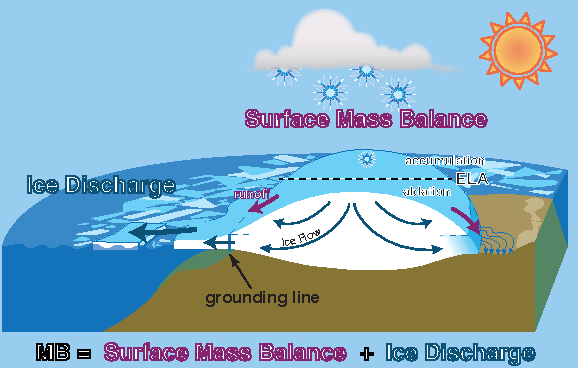
\includegraphics[width=\textwidth]{ice-sheet-cartoon-simple}
  \end{figure}
  \note[item]{explain surface melt, ice discharge/calving, and basal melt}
  \note[item]{snow accumulates in the colder, higher altitude areas in the interior}
  \note[item]{turns into ice}
  \note[item]{and starts to flow downhill towards the coast}
  \note[item]{near the coast, surface melting can occur in the summer}
  \note[item]{but also some ice is dumped directly into the ocean}
  \note[item]{before the mid-90s mass loss was dominated by surface mass balance (80-90\%)}
  \note[item]{contribution of ice discharge was modest (10--20\%)}
  \note[item]{explaining in more detail in the next slide}
\end{frame}


\begin{frame}{Marine Ice Sheet Instability Hypothesis}
  \begin{columns}[c]
    \begin{column}{.65\linewidth}
      \begin{figure}
        \includegraphics<1>[height=8cm]{ant-marine}
      \end{figure}
    \end{column}
    \begin{column}{.38\linewidth}
      \begin{itemize}
      \item blue colors: below sea level
      \end{itemize}
    \end{column}
  \end{columns}
\end{frame}


\setbeamertemplate{background canvas}
{
  \tikz{\node[inner sep=0pt,opacity=1] {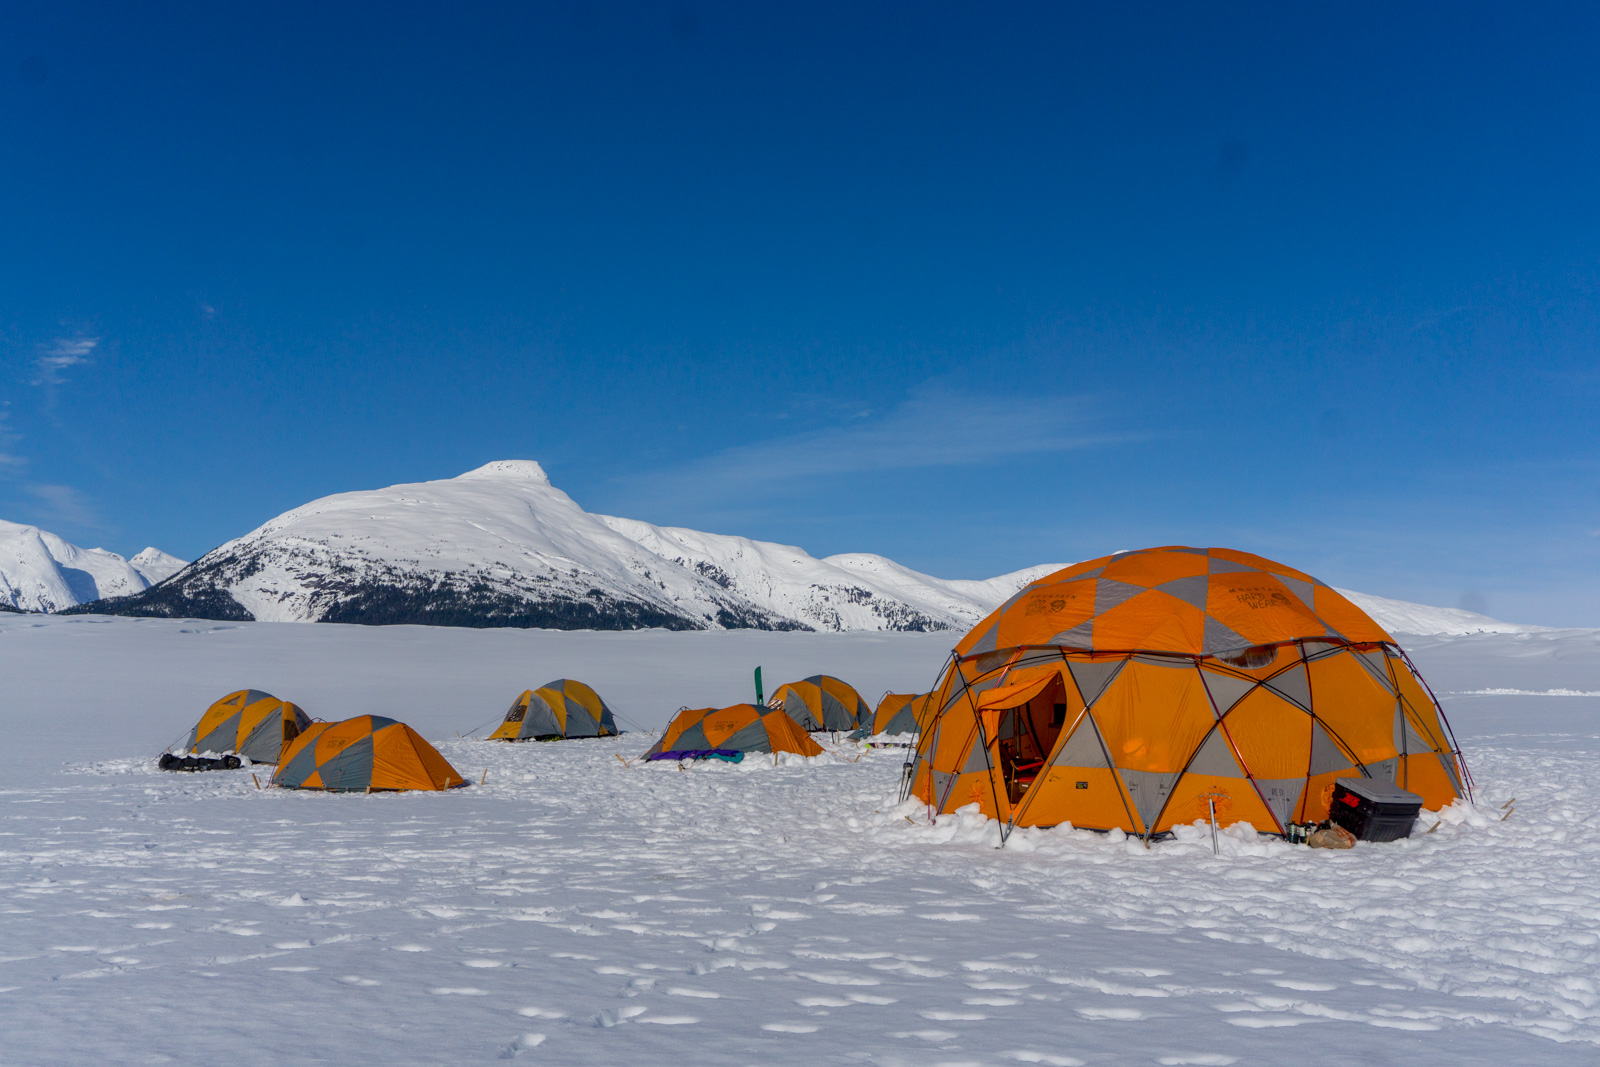
\includegraphics[height=\paperheight,width=\paperwidth]{taku-8}};}
}

\begin{frame}{Questions?}
\end{frame}

\setbeamertemplate{background canvas}
{
}

\begin{frame}{Carbon Dioxide}
      \begin{figure}
        \includegraphics<1>[width=\textwidth]{nasa_co2-graph}
      \end{figure}
\end{frame}


\end{document}

% convert -font Helvetica -pointsize 60 -fill black -draw 'text 1500,080 "1986" ' columbia_0000.jpg columbia_year_0000.jpg
% convert -font Helvetica -pointsize 60 -fill black -draw 'text 1500,080 "1987" ' columbia_0001.jpg columbia_year_0001.jpg
% convert -font Helvetica -pointsize 60 -fill black -draw 'text 1500,080 "1989" ' columbia_0002.jpg columbia_year_0002.jpg
% convert -font Helvetica -pointsize 60 -fill black -draw 'text 1500,080 "1995" ' columbia_0003.jpg columbia_year_0003.jpg 
% convert -font Helvetica -pointsize 60 -fill black -draw 'text 1500,080 "1996" ' columbia_0004.jpg columbia_year_0004.jpg
% convert -font Helvetica -pointsize 60 -fill black -draw 'text 1500,080 "1999" ' columbia_0005.jpg columbia_year_0005.jpg
% convert -font Helvetica -pointsize 60 -fill black -draw 'text 1500,080 "2000" ' columbia_0006.jpg columbia_year_0006.jpg
% convert -font Helvetica -pointsize 60 -fill black -draw 'text 1500,080 "2001" ' columbia_0007.jpg columbia_year_0007.jpg
% convert -font Helvetica -pointsize 60 -fill black -draw 'text 1500,080 "2002" ' columbia_0008.jpg columbia_year_0008.jpg
% convert -font Helvetica -pointsize 60 -fill black -draw 'text 1500,080 "2003" ' columbia_0009.jpg columbia_year_0009.jpg
% convert -font Helvetica -pointsize 60 -fill black -draw 'text 1500,080 "2004" ' columbia_0010.jpg columbia_year_0010.jpg
% convert -font Helvetica -pointsize 60 -fill black -draw 'text 1500,080 "2005" ' columbia_0011.jpg columbia_year_0011.jpg
% convert -font Helvetica -pointsize 60 -fill black -draw 'text 1500,080 "2006" ' columbia_0012.jpg columbia_year_0012.jpg
% convert -font Helvetica -pointsize 60 -fill black -draw 'text 1500,080 "2008" ' columbia_0013.jpg columbia_year_0013.jpg
% convert -font Helvetica -pointsize 60 -fill black -draw 'text 1500,080 "2009" ' columbia_0014.jpg columbia_year_0014.jpg
% convert -font Helvetica -pointsize 60 -fill black -draw 'text 1500,080 "2010" ' columbia_0015.jpg columbia_year_0015.jpg
% convert -font Helvetica -pointsize 60 -fill black -draw 'text 1500,080 "2011" ' columbia_0016.jpg columbia_year_0016.jpg
% convert -font Helvetica -pointsize 60 -fill black -draw 'text 1500,080 "2013" ' columbia_0017.jpg columbia_year_0017.jpg
% convert -font Helvetica -pointsize 60 -fill black -draw 'text 1500,080 "2014" ' columbia_0018.jpg columbia_year_0018.jpg
% convert -font Helvetica -pointsize 60 -fill black -draw 'text 1500,080 "2015" ' columbia_0019.jpg columbia_year_0019.jpg
% convert -font Helvetica -pointsize 60 -fill black -draw 'text 1500,080 "2016" ' columbia_0020.jpg columbia_year_0020.jpg


% resolution=1920x1080
% ffmpeg -y \
%   -framerate 1  \
%   -i columbia_year_%04d.jpg \
%   -s:v $resolution \
%   -c:v libx264  \
%   -crf 20 \
%   -pix_fmt yuv420p \
%   -r 1 \
%   columbia_landsat-hd1920.mp4